\documentclass[10pt]{article}
\usepackage[a4paper,margin=19mm,top=17mm,bottom=18mm]{geometry}
\usepackage[T1]{fontenc}
\usepackage{libertinus}
\usepackage{microtype}
\usepackage{amsmath,mathtools}
\usepackage{amssymb}
\usepackage{booktabs,longtable,tabularx,array,calc}
\usepackage{multicol}
\usepackage{enumitem}
\usepackage{caption}
\usepackage{tikz}
\usetikzlibrary{arrows.meta,positioning,calc,fit,shapes.geometric}
\usepackage{xcolor}
\usepackage{xurl}
\usepackage[hidelinks,hypertexnames=false]{hyperref}
\usepackage{fancyhdr}
\usepackage{titlesec}
\usepackage{needspace}
\usepackage{etoolbox}

\definecolor{heading}{HTML}{111111}
\hypersetup{pdftitle={Permansson Regimes: A General Framework for Strategic Dynamics Beyond Equilibrium},pdfauthor={Marcus Hermansson},pdfsubject={Generated regimes; Permansson regimes; strategic dynamics; intervention-relative constitution}}
\urlstyle{same}
\setcounter{secnumdepth}{0}
\setlength{\parindent}{0pt}
\setlength{\parskip}{4.2pt plus .6pt minus .3pt}
\setlist[itemize]{leftmargin=1.45em,itemsep=1.4pt,topsep=2pt}
\setlist[enumerate]{leftmargin=1.6em,itemsep=1.5pt,topsep=2pt}
\captionsetup{font=small,labelfont=bf,justification=centering}
\renewcommand{\arraystretch}{1.08}
\newcommand{\push}{\mathord{\#}}
\newcommand{\status}[1]{\mbox{\texttt{\scriptsize\detokenize{#1}}}}
\newcommand{\tightlist}{\setlength{\itemsep}{0pt}\setlength{\parskip}{0pt}}
\newcommand{\PaperVersion}{v0.1.8}
\newcommand{\PaperDate}{23 September 2026}
\newcommand{\LeanRepository}{HMarcusWH/PermanssonLean}
\newcommand{\LeanSnapshotCommit}{c018f79ea4ce46f4f679ad5bca254509778fc53c}
\newcommand{\LeanCIRun}{35808810682}
\emergencystretch=2em
\clubpenalty=10000
\widowpenalty=10000
\displaywidowpenalty=10000
\raggedbottom

\titleformat{\section}{\needspace{4\baselineskip}\large\bfseries\color{heading}}{}{0pt}{}
\titleformat{\subsection}{\needspace{3\baselineskip}\normalsize\bfseries\color{heading}}{}{0pt}{}
\titleformat{\subsubsection}{\needspace{2.5\baselineskip}\small\bfseries\color{heading}}{}{0pt}{}
\titlespacing*{\section}{0pt}{10pt plus 2pt minus 1pt}{4pt}
\titlespacing*{\subsection}{0pt}{7pt plus 1pt minus 1pt}{2pt}
\titlespacing*{\subsubsection}{0pt}{6pt plus 1pt minus 1pt}{1.5pt}

\pagestyle{fancy}
\fancyhf{}
\fancyhead[L]{\footnotesize\itshape Permansson Regimes: Strategic Dynamics Beyond Equilibrium}
\fancyfoot[C]{\thepage}
\renewcommand{\headrulewidth}{0.3pt}
\setlength{\headheight}{13pt}

\begin{document}
\begin{center}
{\LARGE\bfseries Permansson Regimes: A General Framework for\\[2pt] Strategic Dynamics Beyond Equilibrium\par}
\vspace{8pt}
{\large Marcus Hermansson\par}
{\small Independent researcher\\Correspondence: \url{https://hmwh.se/}\par}
\vspace{4pt}
{\small Working Paper \PaperVersion{} -- revised \PaperDate\par}
\end{center}
\vspace{3pt}
\section*{Abstract}\label{abstract}

Game-theoretic and learning models often produce a behavioral process whose long-run consequences are then analyzed with tools from dynamical systems, stochastic approximation, occupation measures, or viability theory. The earlier Equilibrium-Generated Regime (EGR) framework formalized a narrower post-equilibrium object: a certified equilibrium policy together with an ex ante regime region, basin, persistence requirement, descriptor, limiting occupation law, convergence mode, and intervention-relative constitutive test. This paper removes equilibrium as a primitive of the regime layer while preserving the strategic semantics that motivated EGR. A canonical strategic-world process separates an action-selection kernel, a world-transition kernel, and a strategic-update kernel; their composition induces an ordinary Markov process on the enlarged state space. Generated Regimes (GRs) are ex ante classifications of that induced process, while generalized Permansson Regimes (PRs) are GRs with at least one strategically constitutive generator component under a fixed admissible intervention. The paper proves well-posedness, exact EGR embedding, conservative recovery of the original Permansson definition, baseline representation invariance, factorization non-identification, and constitutive non-invariance under baseline-equivalent factorizations.

The framework further develops a quantitative and representation-theoretic layer. Descriptor spaces may be Polish; finite persistence and expected exit time admit an exact killed-kernel calculus; finite-horizon quasi-regimes may carry an additional quasi-stationary-distribution (QSD) certificate subject to separate existence and uniqueness conditions; constitutive effects admit a uniform margin and a perturbation-robustness criterion; intervention-compatible invariance extends to frozen intervention families; and a sufficient quotient theorem gives conditions under which GR/PR classification survives type-respecting state compression. These results are modular and apply only under their stated hypotheses. Formal verification and reproducibility materials are documented in Appendix D.

Keywords: generated regimes; Permansson regimes; dynamic games; learning in games; constitutive intervention; killed Markov kernel; quasi-stationary distribution; perturbation robustness; regime equivalence; probabilistic bisimulation.

JEL codes: C72, C73, D02, D74.

\section{1. Introduction}\label{introduction}

\subsection{1.1 The analytical question}\label{the-analytical-question}

A strategic model may identify an equilibrium, a learning rule, an
evolutionary revision protocol, a bounded-rational adjustment process,
or a fixed policy. Once such a process is specified, a second question
remains: what persistent or structurally meaningful world does repeated
strategic behavior generate? In static game theory the natural endpoint
is a solution concept. In dynamic game theory the strategic solution is
coupled to a state process. In evolutionary and learning models the
behavior itself may remain in motion. Across these settings, the world
altered by behavior can in turn reshape future incentives, information,
feasible actions, or strategic updates.

The earlier Equilibrium-Generated Regime framework was built for the
special case in which the strategic behavior was already certified by an
independently established dynamic equilibrium. It deliberately did not
introduce a new equilibrium concept. Instead, it attached a
post-equilibrium classification object to the equilibrium-induced
process: a selected equilibrium policy, an ex ante region and initial
basin, exact persistence, a descriptor, a limiting occupation law, a
convergence mode, and an intervention-relative test for whether a
component of equilibrium behavior was constitutive of a defining regime
property (Hermansson, 2026a).

The present paper asks whether equilibrium was ever logically necessary
to that regime-classification layer. The answer developed here is no,
but only in a specific and conservative sense. The mathematics of
non-equilibrium dynamics is not new: dynamical systems theory classifies
invariant sets, attractors, recurrence, chain recurrence, and related
asymptotic objects; stochastic approximation connects learning
algorithms to differential equations or inclusions; controlled Markov
process theory uses occupation measures; viability theory studies
controlled persistence; evolutionary game theory separates games from
revision protocols; and feedback-evolving games explicitly couple
strategic behavior to environmental states. The proposed contribution is
therefore not a new theory of dynamics. It is a typed, game-facing
regime semantics that preserves the distinction between how strategic
behavior is generated, how that behavior changes the world, and which
typed components are constitutive of a declared regime property.

\subsection{1.2 Main contribution}\label{main-contribution}

The paper introduces a canonical discrete-time strategic-world process
with three kernels. An action-selection kernel \(\alpha\) generates
behavior from the current strategic and world states. A world-transition
kernel P maps current state and behavior into the next world state. A
strategic-update kernel U maps the resulting observation back into the
next strategic state. The pair \(\mathfrak G\) = \((\alpha,U)\) is
called the strategic generator. Their composition induces an ordinary
Markov kernel \(K_{\mathfrak G,P}\) on the joint state Y = S
\(\times{}\) X.

\begin{equation}
Y_t=(S_t,X_t)\xrightarrow{\alpha}A_t\xrightarrow{P}X_{t+1}\xrightarrow{U}S_{t+1}.
\tag{1}\label{eq:1}
\end{equation}

A Generated Regime (GR) is then an ex ante regime specification
satisfied by the induced joint process. A generalized Permansson Regime
(PR) is a GR for which at least one predeclared component of the
strategic generator is constitutive of a defining regime property under
a fixed admissible strategic-generator intervention. Structural
constitution of the world-transition mechanism is defined separately.
For confirmatory use, the framework additionally requires a
nondegenerate baseline specification and a grounded constitutive
property tied to a frozen relevance map; these guardrails exclude
descriptor variation that exists only on unreachable decorative states
and PR claims driven only by undeclared auxiliary bookkeeping
coordinates. This preserves the logic of the earlier EGR paper, in which
a Permansson regime was narrower than an EGR rather than synonymous with
it.


The quantitative and representation-theoretic layer sharpens this architecture in five directions. First, it weakens the descriptor-space assumption from compact metrizable to Polish while preserving the weak-convergence formulation. Second, it replaces the one-step finite-survival diagnostic by an exact killed-kernel calculus, so finite persistence and expected exit time become operator identities rather than only lower bounds. Third, it separates constitutive status from a quantitative constitutive margin and proves a metric perturbation theorem showing exactly when that margin survives model or numerical error. Fourth, it generalizes single-intervention representation invariance to a frozen, indexed intervention-family signature. Fifth, it gives a sufficient quotient theorem: type-respecting state compression preserves GR/PR classification only when both models retain the canonical typed structure, the baseline kernel and every frozen typed intervention kernel intertwine, and the regime/constitutive semantics descend together. None of these results makes perturbation robustness, QSD structure, or quotientability automatic; each applies only under explicit hypotheses.

Formal verification scope and reproducibility provenance are documented in Appendix D.

\begin{figure}[htbp]
\centering
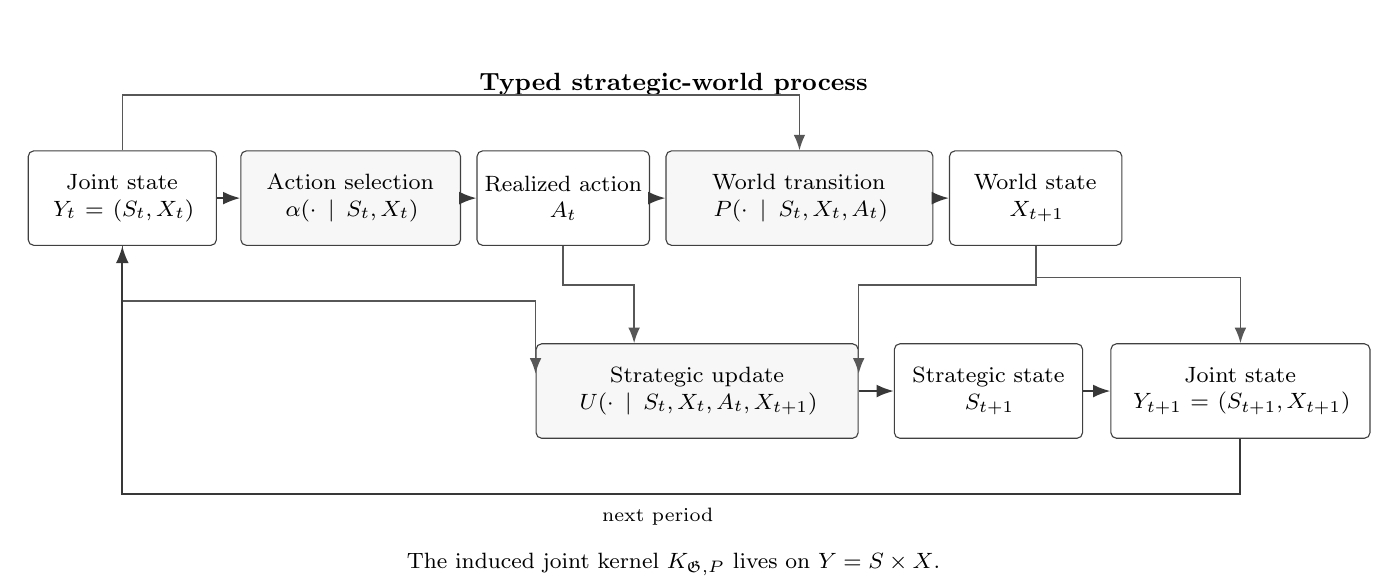
\begin{tikzpicture}[
  >=Latex,
  box/.style={draw=black!75, rounded corners=2pt, fill=white, align=center, minimum height=12mm, inner sep=2.7pt, font=\footnotesize},
  proc/.style={box, fill=black!3},
  arr/.style={->, line width=.72pt, draw=black!78},
  dep/.style={->, line width=.58pt, draw=black!66}
]
\node[font=\small\bfseries] at (7.0,2.55) {Typed strategic-world process};
\node[box, text width=22mm] (yt) at (0,1.1) {Joint state\\$Y_t=(S_t,X_t)$};
\node[proc, text width=26mm] (al) at (2.9,1.1) {Action selection\\$\alpha(\cdot\mid S_t,X_t)$};
\node[box, text width=20mm] (at) at (5.6,1.1) {Realized action\\$A_t$};
\node[proc, text width=32mm] (pw) at (8.6,1.1) {World transition\\$P(\cdot\mid S_t,X_t,A_t)$};
\node[box, text width=20mm] (xp) at (11.6,1.1) {World state\\$X_{t+1}$};

\node[proc, text width=39mm] (up) at (7.3,-1.35) {Strategic update\\$U(\cdot\mid S_t,X_t,A_t,X_{t+1})$};
\node[box, text width=22mm] (sp) at (11.0,-1.35) {Strategic state\\$S_{t+1}$};
\node[box, text width=31mm] (yp) at (14.2,-1.35) {Joint state\\$Y_{t+1}=(S_{t+1},X_{t+1})$};

\draw[arr] (yt.east)--(al.west);
\draw[arr] (al.east)--(at.west);
\draw[arr] (at.east)--(pw.west);
\draw[arr] (pw.east)--(xp.west);

% Additional declared dependencies of P and U.
\draw[dep] (yt.north) -- ++(0,7mm) -| (pw.north);
\draw[dep] (yt.south) -- ++(0,-7mm) -| ([yshift=2.2mm]up.west);
\draw[dep] (at.south) -- ++(0,-5mm) -| ([xshift=-8mm]up.north);
\draw[dep] (xp.south) -- ++(0,-5mm) -| ([yshift=2.2mm]up.east);

\draw[arr] (up.east)--(sp.west);
\draw[arr] (sp.east)--(yp.west);
\draw[dep] (xp.south) -- ++(0,-4mm) -| (yp.north);
\draw[arr] (yp.south) -- ++(0,-7mm) -| (yt.south);
\node[font=\scriptsize, fill=white, inner sep=1pt] at (6.8,-2.95) {next period};

\node[font=\footnotesize] at (7.0,-3.55) {The induced joint kernel $K_{\mathfrak G,P}$ lives on $Y=S\times X$.};
\end{tikzpicture}
\caption{Canonical typed strategic-world process. The joint state $Y_t=(S_t,X_t)$ feeds the action-selection kernel; both the joint state and realized action enter the world transition; and $Y_t$, $A_t$, and $X_{t+1}$ enter the strategic update before $S_{t+1}$ and $X_{t+1}$ recombine as $Y_{t+1}$. The enlarged joint process is ordinary Markov dynamics; the added structure is the declared strategic/world factorization and the intervention semantics.}
\label{fig:typed-process}
\end{figure}

\subsection{1.3 Conservative extension of
EGR}\label{conservative-extension-of-egr}

The set-theoretic relationship requires the intervention grammar to be
typed as well as the baseline object. Let \(\mathrm{PR}_{\iota}\) denote
generalized PR status relative to the transported Paper-I protocol class
introduced in Section 6.3. Recovery of Paper-I objects is assessed on
the embedded EGR class \(\iota(\mathrm{EGR})\). Then:

\begin{equation}
\iota(\mathrm{EGR})\subseteq\mathrm{GR},\qquad \mathrm{PR}_{\mathrm{general}}\subseteq\mathrm{GR},\qquad \mathrm{PR}_{\iota}\subseteq\mathrm{PR}_{\mathrm{general}},\qquad \iota(\mathrm{PR}_{\mathrm{old}})=\iota(\mathrm{EGR})\cap\mathrm{PR}_{\iota}.
\tag{2}\label{eq:2}
\end{equation}

Here \(\iota\) denotes the canonical embedding defined in Section 6. The
restriction to \(\mathrm{PR}_{\iota}\) is essential. The unrestricted
overlap \(\iota(\mathrm{EGR})\cap{}\mathrm{PR}_{\mathrm{general}}\) can
be larger because the generalized theory permits constitutive
interventions on strategic-update or auxiliary-state components that
have no Paper-I policy counterpart. Thus Paper II conservatively
recovers Paper I under transported Paper-I protocols without claiming
that every generalized constitutive property of an embedded
representation existed in Paper I. The framework retains the distinction
between the broad \(\mathrm{PR}_{\mathrm{general}}\) class and grounded
confirmatory PR status: an auxiliary coordinate can support a
confirmatory constitutive claim only when a predeclared relevance map
explicitly includes it. The confirmatory GR layer retains
basin-reachable descriptor nondegeneracy and separately reports whether
descriptor richness remains forward-active after time zero. Conversely,
a non-equilibrium learning process can be a generalized PR if a
component of its strategic generator is constitutive of the declared
regime property. The application-certificate layer leaves these set-theoretic
relations unchanged: empirical provenance, identification, support, or
sampling uncertainty may downgrade an application certificate without
changing the underlying formal GR/PR class.

\begin{figure}[htbp]
\centering
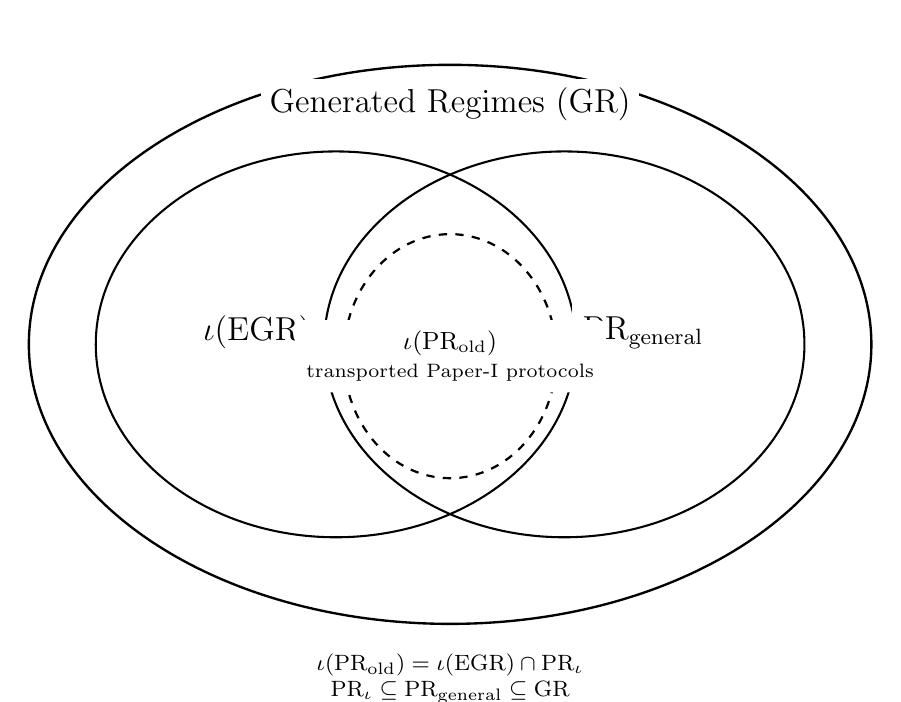
\begin{tikzpicture}[every node/.style={font=\small}]
  \draw[line width=.85pt] (0,0) ellipse (5.35cm and 3.55cm);
  \draw[line width=.75pt] (-1.45,0) ellipse (3.05cm and 2.45cm);
  \draw[line width=.75pt] (1.45,0) ellipse (3.05cm and 2.45cm);
  \draw[dashed,line width=.8pt] (0,-.15) ellipse (1.35cm and 1.55cm);

  \node[fill=white,inner sep=3pt,font=\large] at (0,3.05) {Generated Regimes ($\mathrm{GR}$)};
  \node[fill=white,inner sep=4pt,font=\large] at (-2.45,.15) {$\iota(\mathrm{EGR})$};
  \node[fill=white,inner sep=4pt,font=\large] at (2.45,.15) {$\mathrm{PR}_{\mathrm{general}}$};
  \node[fill=white,rounded corners=2pt,inner sep=4pt,align=center] at (0,-.15) {$\iota(\mathrm{PR}_{\mathrm{old}})$\\[-1pt]{\scriptsize transported Paper-I protocols}};

  \node[fill=white,inner sep=2pt,font=\footnotesize,align=center] at (0,-4.25) {$\iota(\mathrm{PR}_{\mathrm{old}})=\iota(\mathrm{EGR})\cap\mathrm{PR}_{\iota}$\\$\mathrm{PR}_{\iota}\subseteq\mathrm{PR}_{\mathrm{general}}\subseteq\mathrm{GR}$};
\end{tikzpicture}
\caption{Class hierarchy. Transported Paper-I protocol status is denoted $\mathrm{PR}_{\iota}$; exact recovery of Paper-I Permansson regimes is the dashed intersection $\iota(\mathrm{PR}_{\mathrm{old}})$. The unrestricted $\iota(\mathrm{EGR})/\mathrm{PR}_{\mathrm{general}}$ overlap may be larger. The grounded confirmatory subclass $\mathrm{PR}_g\subseteq\mathrm{PR}_{\mathrm{general}}$ is omitted for readability.}
\label{fig:class-hierarchy}
\end{figure}

\subsection{1.4 Scoped novelty claim and
nonclaims}\label{scoped-novelty-claim-and-nonclaims}

The novelty claim is organizational, diagnostic, and semantic rather
than a priority claim over the underlying mathematics. Benaïm and Hirsch
(1996) provide a unified topological framework for limit sets of
asymptotic pseudotrajectories, including fictitious play. Benaïm,
Hofbauer, and Sorin (2005) extend this approach to differential
inclusions. Sandholm (2015) explicitly separates population games from
revision protocols and studies the induced evolutionary dynamics. Weitz
et al. (2016), Tilman, Plotkin, and Akçay (2020), and Ito and Yamamichi
(2024) couple strategic behavior to environmental states and classify
fixed points, bistability, cycles, and related outcomes. Mertikopoulos,
Hsieh, and Cevher (2024) develop a common stochastic-approximation
template for many learning algorithms. Akin (2009), Kloeden and
Rasmussen (2011), and the broader dynamical-systems literature already
supply general asymptotic languages. Aubin (1990) supplies viability and
controlled-invariance machinery. Bhatt and Borkar (1996) characterize
occupation measures in controlled Markov processes.

Accordingly, this paper does not claim: (i) new mathematics of
attractors, recurrence, invariant measures, chain recurrence, or
viability; (ii) a new equilibrium solution concept; (iii) that
strategic/world factorizations are identified from trajectories alone;
(iv) that every persistent trajectory is a GR; (v) that finite-horizon
persistence is equivalent to exact persistence; or (vi) that a signed
feedback diagram by itself provides causal identification. The specific
proposed object is a portable typed regime layer with ex ante
classification and intervention-relative constitutive semantics.

\section{2. Related Literature and the Remaining
Distinction}\label{related-literature-and-the-remaining-distinction}

\subsection{2.1 Population and evolutionary
games}\label{population-and-evolutionary-games}

Population-game theory already contains one of the most important
abstractions for the present paper. Sandholm (2015) models large
populations using revision protocols that generate stochastic
evolutionary processes and deterministic mean dynamics. Fixing a
revision protocol yields a map from population games to differential
equations, and different revision principles can induce qualitatively
different dynamics. This is a direct predecessor of the
strategic-generator idea. The distinction retained here is that the
generated behavior is subsequently composed with an explicitly typed
world-transition mechanism and then classified by a regime specification
that remains unchanged across admissible generator classes.

Arcak and Martins (2021) offer another close architectural analogue by
separating a payoff dynamics model from an evolutionary dynamics model
and studying stability compositionally. Their target is convergence to
Nash-like rest points under dissipativity conditions. The present
framework instead treats convergence, cycles, invariant occupation laws,
or other declared regime forms as possible outputs, and it preserves a
separate constitutive intervention grammar.

\subsection{2.2 Learning and stochastic
approximation}\label{learning-and-stochastic-approximation}

Learning in games provides a large family of non-equilibrium generators.
Mertikopoulos, Hsieh, and Cevher (2024) develop a unified
stochastic-approximation template spanning gradient methods,
multiplicative weights, optimistic methods, bandit methods, and related
algorithms. Benaïm and Hirsch (1996) and Benaïm, Hofbauer, and Sorin
(2005) show how broad adaptive processes can be analyzed through
internally chain-recurrent or internally chain-transitive limit sets.
Galla and Farmer (2013) show that reinforcement-learning dynamics in
complicated games can exhibit fixed points, multiplicity, limit cycles,
and high-dimensional chaos. Milionis et al. (2023) prove an
impossibility result showing that Nash convergence cannot be a universal
requirement for game dynamics.

These results strongly motivate separating generator type from regime
type. A learning generator may produce a fixed point, cycle, chaotic
attractor, or invariant distribution depending on the model.
``Non-equilibrium'' is therefore not itself a regime classification. It
is a statement about the generator or the absence of a particular
solution certificate.

\subsection{2.3 Strategy-environment
feedback}\label{strategy-environment-feedback}

Feedback-evolving games are the closest substantive game-facing
neighbor. Weitz et al. (2016) explicitly model accumulated strategic
behavior as changing the commons and thereby changing subsequent
payoffs. Tilman, Plotkin, and Akçay (2020) generalize the framework by
separating intrinsic environmental dynamics, strategic impact on the
environment, and strategy-update dynamics. Ito and Yamamichi (2024)
provide a broad qualitative classification for feedback-evolving games,
including stable equilibria, bistability, transient changes in game
structure, and persistent oscillation.

These models already establish the conceptual legitimacy of strategic
behavior \(\leftrightarrow\) world feedback and of regime-like
qualitative classification. The remaining distinction is portability:
the canonical feedback-evolving model is usually tied to a specific
evolutionary update equation or family. The present paper instead treats
the strategic generator as a typed replaceable input while keeping the
regime specification and constitutive semantics fixed.

\subsection{2.4 Dynamical systems and the enlarged-state
objection}\label{dynamical-systems-and-the-enlarged-state-objection}

The strongest reduction argument against the present framework is
mathematically correct: set \(Y_t=(S_t,X_t)\), forget the interpretation
of the factors, and analyze the induced process with ordinary
dynamical-systems or Markov-process tools. Akin's survey develops
invariant sets, attractors, chain recurrence, Lyapunov functions,
minimality, and recurrence. Benaïm and Hirsch characterize limit sets of
broad nonautonomous pseudotrajectories. Kloeden and Rasmussen develop
nonautonomous processes, pullback attractors, switching systems, and
random dynamical systems. Conley-theoretic reasoning also enters modern
game dynamics, as emphasized by Milionis et al. (2023).

This paper accepts that reduction at the level of baseline dynamics. Its
claim is that the reduction loses information required for constitutive
questions. If two different strategic/world factorizations induce the
same K, they are dynamically indistinguishable at baseline. Yet an
intervention on the strategic generator may leave one K unchanged and
alter the other. The factorization is therefore irrelevant to baseline
dynamical classification but relevant to typed counterfactual
constitution. Sections 6 and 7 formalize this distinction.

\subsection{2.5 Viability, controlled Markov processes, and
institutions}\label{viability-controlled-markov-processes-and-institutions}

Viability theory provides mature mathematics for remaining inside
declared sets under control and for computing viability kernels and
capture basins (Aubin, 1990). Controlled Markov process theory similarly
provides policy-induced occupation measures and long-run state-action
structure (Bhatt and Borkar, 1996). These are important mathematical
substrates for particular GR descriptors and persistence criteria rather
than competing vocabularies that must be replaced.

Institutional theory supplies a conceptual analogue at a different
level. Greif and Laitin (2004) ask how self-enforcing institutions
persist in changing environments and how processes unleashed by
institutions can reinforce or undermine them. Their quasi-parameter and
self-reinforcement concepts are closely related to the idea that
behavior changes a world state that feeds back into future strategic
conditions. The present framework aims to provide a more abstract
process-and-intervention language that can host such mechanisms without
identifying institutions with equilibrium by definition.

\subsection{2.6 Causal abstraction and causal games}\label{causal-abstraction-and-causal-games}

Causal abstraction provides the closest existing formal language for the
intervention-sensitive equivalence problem underlying Sections 7.2--7.4.
Rubenstein et al. (2017) introduce exact transformations between structural
equation models and explicitly require agreement about the effects of mapped
interventions across levels of description. Beckers and Halpern (2019) refine
this idea through increasingly restrictive notions of causal abstraction;
Otsuka and Saigo (2022) give a category-theoretic equivalence criterion under
which intervention calculi translate consistently; and Geiger et al. (2025)
generalize causal abstraction from mechanism replacement to broader mechanism
transformations. These results already establish that representation-level or
baseline agreement is not by itself the relevant notion of equivalence when
interventions matter.

Causal games bring that same issue directly into strategic settings. Hammond
et al. (2023) define structural causal games with mechanised representations of
decision rules and provide prediction, intervention, and counterfactual
semantics. Mishra, Fox, and Wooldridge (2024) further characterize primitive
interventions in causal games, including distinctions that determine whether
agents may adapt their policies after an intervention. These literatures
therefore substantially anticipate the general intervention-sensitive
principle used here. What remains distinct is not intervention semantics
itself, but the Generated-Regime object: a reusable ex ante persistent-regime
specification that can be applied across heterogeneous strategic generators,
together with the Permansson subclass whose membership is defined by
constitutive strategic intervention response. The present framework should
therefore be read as a regime-classification layer compatible with causal
abstraction and causal-game machinery, not as a replacement for either.


\subsection{2.7 Labelled Markov processes, killed processes, and perturbation theory}\label{labelled-killed-perturbation}

Labelled Markov-process theory is the closest process-theoretic prior art for the intervention-family layer. Desharnais et al. (2004) construct behavioral metrics whose zero set is bisimilarity, while Danos et al. (2006) formulate event bisimulation through sub-$\sigma$-algebras on general measurable spaces. These results already establish that families of transition kernels indexed by labels admit exact and approximate behavioral equivalence notions. The contribution here is therefore not the generic idea of a label-indexed kernel family; it is the sufficient bridge from a frozen family of typed strategic interventions to GR/PR regime and constitution statements.

Killed-process theory supplies the exact finite-survival and quasi-stationary machinery used in Section 4. Bena\"im, Cloez, and Panloup (2018) analyze quasi-stationary distributions for killed Markov processes on compact spaces, while Coolen-Schrijner and van Doorn (2006) and van Doorn and Pollett (2009) demonstrate why QSD existence, uniqueness, and limiting conditional behavior require separate hypotheses. The present paper uses only the elementary sub-Markov identities universally; QSD claims are optional certified subclasses.

Finally, the quantitative layer draws on established perturbation theory rather than presenting a universal new sensitivity theorem. Mitrophanov (2005) derives perturbation bounds for uniformly ergodic Markov chains, and Rudolf and Wang (2025) quantify stability of quasi-stationary laws for killed processes under generator perturbations. Such results enter only as subclass inputs; the general theorem here is the metric margin bridge from bounded property-output error to preserved constitutive classification.

\begin{table}[htbp]
\centering
\footnotesize
\caption{Closest neighboring literatures. The framework deliberately uses established mathematical objects where possible; the proposed addition is the typed regime and intervention layer.}
\label{tab:literature-neighbors}
\begin{tabularx}{\textwidth}{@{}>{\raggedright\arraybackslash}p{.18\textwidth}>{\raggedright\arraybackslash}p{.22\textwidth}>{\raggedright\arraybackslash}p{.25\textwidth}>{\raggedright\arraybackslash}X@{}}
\toprule
\textbf{Literature} & \textbf{Generator / process} & \textbf{Persistent object} & \textbf{What remains distinct here}\\
\midrule
Population games & Revision protocols & Rest points, convergence, cycles, stochastic stability & Separate world kernel and portable regime/intervention semantics\\
Learning in games & Broad learning algorithms & Attractors, limit sets, invariant measures & Same GR definition across generator classes\\
Feedback-evolving games & Usually replicator / evolutionary updates & Fixed points, bistability, cycles & Generator replacement plus typed constitution\\
Dynamical systems & Arbitrary law on enlarged state & Invariant sets, recurrence, attractors & Strategic/world semantics and intervention type\\
Causal abstraction / causal games & Structural mechanisms, decision rules, typed interventions & Intervention-preserving equivalence; causal/counterfactual predictions & Portable persistent-regime object and PR membership rule\\
Labelled Markov / bisimulation & Label-indexed transition kernels & Behavioral equivalence and metrics & Typed intervention-family signature plus GR/PR semantic preservation\\
Killed / quasi-stationary processes & Sub-Markov kernels and absorption & Survival, exit laws, QSDs & Exact finite-persistence calculus with optional QSD certification of quasi-regimes\\
Markov perturbation theory & Baseline/perturbed kernels & Sensitivity of finite or long-run laws under hypotheses & Property-output error bridge to constitutive classification\\
Controlled Markov / viability & Policies or controls & Occupation measures, viable sets, capture basins & Game-facing regime property and constitutive decomposition\\
Endogenous institutions & Case-specific repeated-game mechanisms & Persistence, reinforcement, endogenous change & Portable process-level formalization\\
\bottomrule
\end{tabularx}
\end{table}

\section{3. Canonical Strategic-World
Environment}\label{canonical-strategic-world-environment}

\subsection{3.1 Measurable spaces and
states}\label{measurable-spaces-and-states}

The canonical paper uses discrete time t \(\in{}\) \(\mathbb N_0\) and a
Markovian representation. Continuous-time, differential-inclusion, and
nonautonomous extensions are discussed later. Let (S, B(S)) and (X,
B(X)) be nonempty Polish spaces representing the strategic state and the
world state. Let \(Y=S\times{}X\) with the product Borel
\(\sigma\)-algebra. Where a measure-based non-triviality test is used,
fix a nonzero Borel reference measure m on Y as part of the model before
any regime region is declared. The strategic state may include policies,
learning weights, beliefs, memory variables, population strategy
frequencies, internal organizational rules, or other variables required
to generate future behavior. The world state contains the material,
institutional, environmental, network, informational, or other state
altered through behavior.

The decomposition is analytical rather than ontological. If a variable
is required to make the mechanism Markovian, it must be included in S or
X. If a distinction cannot be empirically identified, the model may
still declare it structurally, but Section 7 shows that the
factorization is not generally identified from the induced joint
process.

\subsection{3.2 Actions and feasibility}\label{actions-and-feasibility}

Let \(I=\{1,\ldots,n\}\) be a finite player set when a multi-player
interpretation is available. For each player i, let \(A_i\) be a
nonempty standard Borel action space and let \(A_i(y)\subseteq{}A_i\) be
a nonempty feasible-action correspondence with measurable graph. Let
\(A=\prod_i\) \(A_i\) and \(A(y)=\prod_i\) \(A_i(y)\). For a
single-agent, population-level, or exogenous formulation, take A
directly to be any nonempty standard Borel behavioral-output space with
a nonempty measurable feasible correspondence A(y).

\subsection{3.3 The strategic generator}\label{the-strategic-generator}

The strategic generator is the ordered pair

\begin{equation}
\mathfrak G=(\alpha,U).
\tag{3}\label{eq:3}
\end{equation}

The action-selection kernel \(\alpha(da\mid s,x)\) is a Markov kernel
from \(Y\) to \(A\) satisfying feasibility:

\begin{equation}
\alpha\!\left(A(s,x)\mid s,x\right)=1\qquad\text{for every }(s,x)\in Y.
\tag{4}\label{eq:4}
\end{equation}

The strategic-update kernel \(U(ds'\mid s,x,a,x')\) is a Markov kernel
from \(S\times{}X\times{}A\times{}X\) to \(S\). It updates the internal
strategic state after the action and the realized next world state are
available. This ordering is intentionally more general than a single
kernel \(\Gamma(da,ds'\mid s,x)\): learning rules often update beliefs,
propensities, or policies only after observing consequences, rewards, or
public signals. Any additional observation can be included explicitly or
encoded in the augmented next state.

\subsection{3.4 World transition}\label{world-transition}

Let \(P(dx'\mid s,x,a)\) be a Markov kernel from \(Y\times{}A\) to X.
Only its values on feasible state-action pairs matter because \(\alpha\)
is supported on A(s,x). If an application initially specifies a kernel
only on the Borel feasible graph, fix a measurable extension off that
graph before applying the canonical formulas; because X is nonempty, a
fixed probability law on X can be used off the feasible graph. P
contains both intrinsic world dynamics and action-dependent
consequences. In a game-environment model, for example, P may encode
resource renewal together with depletion caused by current behavior. In
an institutional model it may encode how actions alter operative rules,
status, capacity, or other continuation-relevant state.

\subsection{3.5 Induced joint kernel}\label{induced-joint-kernel}

For a measurable rectangle \(C\times{}D\subseteq{}S\times{}X\) define

\begin{equation}
K_{\mathfrak G,P}(C\times D\mid s,x)=\int_A\!\int_D U(C\mid s,x,a,x')\,P(dx'\mid s,x,a)\,\alpha(da\mid s,x).
\tag{5}\label{eq:5}
\end{equation}

Equivalently, for any \(E\in{}B(Y)\),

\begin{equation}
K_{\mathfrak G,P}(E\mid s,x)=\int_A\!\int_X\!\int_S \mathbf 1_E(s',x')\,U(ds'\mid s,x,a,x')\,P(dx'\mid s,x,a)\,\alpha(da\mid s,x).
\tag{6}\label{eq:6}
\end{equation}

\textbf{Theorem 3.1 (Joint-process well-posedness).} Under the
measurability and feasibility assumptions above, \(K_{\mathfrak G,P}\)
is a Markov kernel on \(Y\). For every initial law
\(\lambda_0\in{}\Delta(Y)\), there exists a unique probability law
\(P^{\mathfrak G,P}_{\lambda_0}\) on \(\Omega=Y^{\mathbb N_0}\) whose
canonical coordinate process has initial law \(\lambda_0\) and
transition kernel \(K_{\mathfrak G,P}\).

\emph{Proof.} Kernel measurability follows from standard composition of
measurable kernels: first integrate the bounded measurable indicator
\(\mathbf 1_E(s',x')\) against U, then P, then \(\alpha\). The resulting
map \(y\mapsto{}K(E\mid y)\) is measurable for every Borel E, and
\(K(Y\mid y)=1\). Since S and X are Polish, \(Y=S\times{}X\) is Polish
and hence standard Borel. Ionescu-Tulcea then yields a unique
probability measure on the countable product path space with the stated
initial law and transition kernel. \hfill\textsc{q.e.d.}

\textbf{Proposition 3.2 (Enlarged-state reduction).} Every canonical
strategic-world model is an ordinary Markov process on the enlarged
state \(Y=S\times{}X\). Consequently, every baseline property that
depends only on the induced path law can, in principle, be studied
without retaining the strategic/world factorization.

\emph{Proof.} Immediate from Theorem 3.1. The proposition is a
reduction, not a novelty claim. Its importance is diagnostic: any
claimed contribution of the typed factorization must concern semantics
or interventions not recoverable from K alone. \hfill\textsc{q.e.d.}

\begin{table}[htbp]
\centering
\small
\caption{Core notation.}
\label{tab:notation}
\begin{tabularx}{\textwidth}{@{}>{\raggedright\arraybackslash}p{.28\textwidth}X@{}}
\toprule
\textbf{Symbol} & \textbf{Meaning}\\
\midrule
$S_t$ & Strategic state\\
$X_t$ & World state\\
$Y_t=(S_t,X_t)$ & Joint state\\
$A_t$ & Realized strategic behavior\\
$\alpha$ & Action-selection kernel\\
$U$ & Strategic-update kernel\\
$\mathfrak G=(\alpha,U)$ & Strategic generator\\
$P$ & World-transition kernel\\
$K_{\mathfrak G,P}$ & Induced joint kernel on $Y$\\
$P_{\lambda}^{\mathfrak G,P}$ & Induced path law from initial law $\lambda$\\
$\Delta(E)$ & Borel probability measures on measurable space $E$\\
$f_{\push}\mu$ & Pushforward of $\mu$ under measurable map $f$\\
$\delta_y$ & Dirac probability law at $y$\\
$B$ & Predeclared regime region\\
$B_0$ & Predeclared initial basin\\
$B_1$ & Predeclared constitutive comparison set\\
$h$ & Regime descriptor\\
$\nu$ & Limiting occupation law\\
$\mathfrak c$ & Declared convergence mode\\
$g$ & Frozen relevance map for grounded confirmatory use\\
$\psi$ & Defining regime-property map\\
$d_\psi$ & Metric on the property space $Z_\psi$\\
$J$ & Typed admissible intervention\\
$m$ & Reference measure for non-triviality test\\
$K_B$ & Killed/sub-Markov kernel obtained by restricting $K$ to transitions remaining in $B$\\
$\Delta_{\psi,J}(y)$ & Pointwise constitutive effect distance under intervention $J$\\
$\kappa_{\psi,J}(B_1)$ & Uniform constitutive margin: infimum of $\Delta_{\psi,J}$ over $B_1$\\
$\operatorname{Sig}_{\mathcal J}(M)$ & Frozen indexed baseline-plus-intervention kernel signature for family $\mathcal J$\\
\bottomrule
\end{tabularx}
\end{table}

\section{4. Generated Regimes}\label{generated-regimes}

\subsection{4.1 Ex ante regime
specification}\label{ex-ante-regime-specification}

Let H be a Polish descriptor space. Fix a bounded compatible metric
\(d_H\) on H---for example, replace any compatible complete metric \(\rho\) by
\(\min\{1,\rho\}\)---and let \(d_{\mathrm{BL}}\) be the corresponding
bounded-Lipschitz/Fortet--Mourier metric on \ensuremath{\Delta(H)}. On a Polish space,
\(d_{\mathrm{BL}}\) metrizes weak convergence of probability measures (Dudley, 2002). A
regime specification is

\begin{equation}
\Sigma=(B,B_0,h,\nu,\mathfrak c).
\tag{7}\label{eq:7}
\end{equation}

where \(B_0\subseteq{}B\subseteq{}Y\) are Borel sets, \(h:Y\to{}H\) is
Borel measurable, \(\nu\in{}\Delta(H)\), and \(\mathfrak c\) records the
declared convergence mode. The descriptor is defined on all of Y rather
than only on B so that the same map remains evaluable under
interventions that may force exit from the baseline region.

\textbf{Proposition 4.1a (Polish descriptor-space generality).} Replacing compact metrizability of H by Polishness leaves every definition in Sections 4--7 well posed. In particular, a bounded compatible metric exists, \(\Delta(H)\) is metrizable by \(d_{\mathrm{BL}}\) for weak convergence, and the occupation-law conditions below remain meaningful. Polishness alone does not imply uniform tightness of an arbitrary sequence of occupation laws and does not imply existence of a limiting law.

\emph{Proof.} Let \(\rho\) be any compatible complete separable metric on H and set \(d_H=\min\{1,\rho\}\). This bounded metric generates the same topology. The associated bounded-Lipschitz metric metrizes weak convergence on probability measures over a Polish space. The remaining definitions use only Borel measurability of h, probability laws on H, and the declared convergence mode. No compactness step is invoked. A sequence of probability measures on a noncompact Polish space need not be uniformly tight, so existence of \(\nu\) remains an Exact-GR requirement rather than a consequence of the ambient topology. \hfill\textsc{q.e.d.}

Define the admissible initial-law class

\begin{equation}
\mathcal D(B_0)=\{\lambda\in\Delta(Y):\lambda(B_0)=1\}.
\tag{8}\label{eq:8}
\end{equation}

The specification is analyst-relative and is not uniquely determined by
the process. To block post hoc regime drawing, the following ex ante
non-triviality conditions are imposed. For confirmatory certification, a
stronger process-relevant descriptor check is added immediately
afterward.

Assumption 4.1 (Ex ante non-triviality). (i) \(B_0\) and B are Borel
with nonempty \(B_0\subseteq{}B\). (ii) The regime region B has nonempty
interior or positive measure under the reference measure m fixed with
the model before B is declared. (iii) h(B) contains at least two points.
(iv) \(B_0\) contains at least two states that induce distinct baseline
path laws. (v) B, \(B_0\), h, \(\nu\), and \(\mathfrak c\) are declared
before the evaluated trajectory is classified. The same h is used in
baseline and intervention comparisons.

Because a point-initialized path law on $\Omega=Y^{\mathbb N_0}$ includes the deterministic coordinate $Y_0=y$, condition (iv) is literally equivalent to requiring at least two distinct initial states; it blocks singleton basins but does not by itself guarantee different continuation dynamics. Shifted continuation-law diversity $P_y\circ\theta^{-1}\ne P_{y'}\circ\theta^{-1}$, where $\theta(y_0,y_1,\ldots)=(y_1,y_2,\ldots)$, remains a useful strengthening diagnostic. For grounded confirmatory work, an additional optional response-profile diagnostic may compare the $g$-projected baseline and frozen-intervention path laws: two states can be substantively distinguishable if their grounded law differs at baseline or under the declared intervention. Neither baseline grounded diversity nor shifted-law diversity is a universal theorem precondition, because latent types, beliefs, or learning states may pool at baseline while responding differently to the counterfactual, and contraction-to-attractor regimes may lose forward diversity immediately. Condition (v) does not prohibit exploratory model development, but exploratory regions must be frozen and evaluated on held-out simulations, data, or cases before confirmatory classification. For confirmatory certification, define the basin-reachable descriptor-law family
\[
\mathcal M_h(B_0)=\bigl\{h_{\push}(\delta_y K_{\mathfrak G,P}^{t}):y\in B_0,\ t\in\mathbb N_0\bigr\}.
\]
A specification is called descriptor-nondegenerate when $\mathcal M_h(B_0)$ contains at least two distinct probability measures. This blocks an unreachable decorative state from supplying all descriptor variation. A stronger diagnostic is forward descriptor richness: let $R_h^+(B_0)$ be the closure in $H$ of the union of $\operatorname{supp}(h_{\push}(\delta_y K_{\mathfrak G,P}^{t}))$ over $y\in B_0$ and integers $t\ge1$; the specification is forward-descriptor-rich when $R_h^+(B_0)$ contains at least two points. Forward richness is not a universal certification gate. A one-step contraction from a nontrivial basin to a common fixed point can be a perfectly legitimate Exact GR. Confirmatory reports should therefore state whether nondegeneracy is forward-active or basin-only; basin-only status is not a failure, but it should not be described as persistent descriptor variation.

\subsection{4.2 Exact and finite-horizon
persistence}\label{exact-and-finite-horizon-persistence}

Define the first exit time

\begin{equation}
\tau_B=\inf\{t\ge 0:Y_t\notin B\}.
\tag{9}\label{eq:9}
\end{equation}

The regime region is exactly invariant under \(K_{\mathfrak G,P}\) when

\begin{equation}
K_{\mathfrak G,P}(B\mid y)=1\qquad\text{for every }y\in B.
\tag{10}\label{eq:10}
\end{equation}

\textbf{Proposition 4.2 (Equivalent forms of exact invariance).} For a
Markov process with kernel \(K_{\mathfrak G,P}\), condition (10) is
equivalent to \(P^{\mathfrak G,P}_y(\tau_B=\infty)=1\) for every
\(y\in{}B\).

\emph{Proof.} If $K(B\mid y)=1$ on $B$, induction gives $P_y(Y_t\in B\text{ for all }t\le T)=1$ for every finite $T$. Countable intersection over $T$ yields indefinite retention almost surely. Conversely, if indefinite retention holds from every $y\in B$, then in particular $P_y(Y_1\in B)=K(B\mid y)=1$. \hfill\textsc{q.e.d.}

For \(L\in\mathbb N\) and \(\eta\in{}[0,1]\), define \((L,\eta)\)-persistence
by

\begin{equation}
\inf_{y\in B} P_y^{\mathfrak G,P}(\tau_B>L)\ge 1-\eta.
\tag{11}\label{eq:11}
\end{equation}

For measurable B define the killed (sub-Markov) kernel on B by

\begin{equation}
K_B(y,C)=K_{\mathfrak G,P}(C\cap B\mid y),\qquad y\in B,\ C\in\mathcal B(Y).
\tag{11a}\label{eq:11a}
\end{equation}

The killed kernel records exactly the mass that remains in B after each transition; missing mass is the probability already absorbed at the cemetery state.

\textbf{Theorem 4.2a (Exact killed-kernel persistence calculus).} For every \(y\in B\) and integer \(n\ge0\),

\begin{equation}
P_y^{\mathfrak G,P}(\tau_B>n)=\bigl(K_B^n\mathbf 1_B\bigr)(y).
\tag{11b}\label{eq:11b}
\end{equation}

Moreover, with values in \([0,\infty]\),

\begin{equation}
E_y^{\mathfrak G,P}[\tau_B]=\sum_{n=0}^{\infty}\bigl(K_B^n\mathbf 1_B\bigr)(y).
\tag{11c}\label{eq:11c}
\end{equation}

\emph{Proof.} Because \(y\in B\), the event \(\{\tau_B>n\}\) is exactly \(\{Y_1\in B,\ldots,Y_n\in B\}\). For \(n=0\) both sides equal one. If the identity holds at n, the Markov property gives
\[
P_y(\tau_B>n+1)=\int_B P_z(\tau_B>n)\,K_{\mathfrak G,P}(dz\mid y)=\bigl(K_B^{n+1}\mathbf 1_B\bigr)(y),
\]
proving (11b) by induction. Equation (11c) is the tail-sum identity for a nonnegative integer-valued random variable, with monotone convergence allowing the value \(+\infty\). \hfill\textsc{q.e.d.}

\textbf{Corollary 4.2b (Exact finite-persistence characterization).} Condition (11) is equivalent to

\begin{equation}
\inf_{y\in B}\bigl(K_B^L\mathbf 1_B\bigr)(y)\ge 1-\eta.
\tag{11d}\label{eq:11d}
\end{equation}

\textbf{Corollary 4.2c (One-step lower bound).} If \(K_{\mathfrak G,P}(B\mid y)\ge q\) for every \(y\in B\), then \((K_B^L\mathbf 1_B)(y)\ge q^L\) for every \(y\in B\). This is a lower bound on the exact quantity (11d), not a replacement for it, and when \(q<1\) it supplies no positive lower bound on indefinite survival.

Finite-horizon survival remains strictly weaker than exact persistence. Equations (11b)--(11d) identify the exact finite-horizon object; Proposition 4.2 continues to characterize the separate exact-invariance boundary. The labels exact GR, quasi-regime, and metastable extension are therefore kept distinct.

\subsection{4.3 Descriptors and limiting occupation
laws}\label{descriptors-and-limiting-occupation-laws}

For the descriptor process \(h(Y_t)\), define the empirical occupation
measure

\begin{equation}
\widehat\nu_T^{\,h}=\frac{1}{T}\sum_{t=0}^{T-1}\delta_{h(Y_t)}.
\tag{12}\label{eq:12}
\end{equation}

The canonical convergence modes are:

\begin{itemize}
\item
  Almost sure weak convergence:
  \(d_{\mathrm{BL}}(\widehat\nu_T^h,\nu)\to{}0\) almost surely for every
  \(\lambda_0\in{}\mathcal D(B_0)\).
\item
  Convergence in probability under \(d_{\mathrm{BL}}\): for every
  \(\varepsilon>0\),
  \(P(d_{\mathrm{BL}}(\widehat\nu_T^h,\nu)>\varepsilon)\to{}0\) for
  every admissible \(\lambda_0\).
\item
  Mean bounded-Lipschitz convergence:
  \(E[d_{\mathrm{BL}}(\widehat\nu_T^h,\nu)]\to{}0\) for every admissible
  \(\lambda_0\).
\item
  Convergence in distribution of the random occupation measure:
  \(\widehat\nu_T^h\) \(\Rightarrow{}\) \(\nu\) as random elements of
  \ensuremath{\Delta(H)}, equivalently \(\mathcal L(\widehat\nu_T^h)\Rightarrow\delta_\nu\).
  Because the target \(\nu\) is deterministic and \ensuremath{\Delta(H)} is metrizable,
  this mode is equivalent to convergence in probability to \(\nu\); it
  is listed explicitly to preserve the Paper-I convergence vocabulary.
\item
  These modes are canonical rather than exhaustive: \(\mathfrak c\) may
  specify another precisely defined convergence mode, provided the mode
  is fixed ex ante and is meaningful for every admissible initial law.
\end{itemize}

A limiting occupation law is not automatically an invariant law of a
Markov factor. Call h a Markov factor for \(K_{\mathfrak G,P}\) on B if
there exists a Markov kernel \(K_h\) on H such that
\(K_{\mathfrak G,P}(h^{-1}(C)\mid y)=K_h(C\mid h(y))\) for every
\(y\in{}B\) and every Borel \(C\subseteq{}H\). Only when such a factor
kernel is available and \(\nu{}K_h=\nu\) is \(\nu\) called invariant on
the factor space; otherwise \(\nu\) remains an occupation-law descriptor
of the full process.

Definition 4.3 (Exact Generated Regime). An Exact Generated Regime is a
tuple \(R=(\mathfrak G,P,B,B_0,h,\nu,\mathfrak c)\) such that: (i) the
canonical process is well posed; (ii) Assumption 4.1 holds; (iii) B is
exactly invariant under \(K_{\mathfrak G,P}\); and (iv) \(\nu\) is a
limiting occupation law for every \(\lambda_0\in{}\mathcal D(B_0)\) under the
declared convergence mode \(\mathfrak c\). An Exact GR is called
descriptor-nondegenerate when, in addition, the basin-reachable
descriptor-law family \(\mathcal M_h(B_0)\) defined above contains at least two
distinct measures. Confirmatory GR certification in this paper uses the
descriptor-nondegenerate subclass; the broader Exact-GR definition is
retained for exact backward compatibility with Paper I. Forward-descriptor-rich
status is a separately reported stronger diagnostic, not an additional
universal gate.

Common admissible descriptors include fixed-point or periodic factor
dynamics, recurrence classes, occupation shares, balanced growth after
normalization, contraction, approach to a target set, or a finite
symbolic regime code. Labels such as ``stable,'' ``chaotic,''
``self-reinforcing,'' or ``transitioning'' must be tied to explicit
topological, probabilistic, or intervention-relative conditions rather
than used as free interpretive adjectives.

\subsection{4.4 Quasi-regimes and metastable
extensions}\label{quasi-regimes-and-metastable-extensions}

An \((L,\eta)\)-quasi-regime freezes the same ex ante
region/basin/descriptor specification and satisfies the finite-horizon
survival bound (11), but it is not an Exact GR and need not possess a
limiting occupation law unless that is established separately. A
metastable GR extension additionally declares a disturbance or
approximation family \(\{K_\varepsilon\}_{\varepsilon>0}\), a region B,
a basin \(B_0\), and an integer-valued exit-time scale
\(r:(0,\varepsilon_0]\to{}N\) with \(r(\varepsilon)\to{}\infty\) as
\(\varepsilon\downarrow0\). A minimal metastability requirement is

\begin{equation}
\lim_{\varepsilon\downarrow 0}\;\inf_{y\in B_0}P_y^{K_\varepsilon}\!\left(\tau_B>r(\varepsilon)\right)=1.
\tag{13}\label{eq:13}
\end{equation}

This definition is intentionally weak and is not presented as a universal metastability concept. An optional stronger subclass based on killed-process theory is defined next, while remaining separate from Exact GR.

\textbf{Definition 4.4a (QSD-certified quasi-regime).} An \((L,\eta)\)-quasi-regime is QSD-certified by a pair \((\mu_B,\theta_B)\) if, in addition to satisfying the finite-persistence gate (11), its killed kernel \(K_B\) admits a probability measure \(\mu_B\) on B and a survival factor \(\theta_B\in(0,1]\) such that

\begin{equation}
\mu_B K_B=\theta_B\mu_B.
\tag{13a}\label{eq:13a}
\end{equation}

The eigenmeasure relation (13a) is an additional certificate for the killed dynamics; by itself it does not imply the uniform statewise finite-persistence requirement in (11).

\textbf{Proposition 4.4b (QSD survival and conditional stationarity).} If (13a) holds, then for every \(n\ge0\),

\begin{equation}
P_{\mu_B}(\tau_B>n)=\theta_B^n,\qquad \mathcal L(Y_n\mid\tau_B>n)=\mu_B.
\tag{13b}\label{eq:13b}
\end{equation}

\emph{Proof.} Iterating (13a) gives \(\mu_BK_B^n=\theta_B^n\mu_B\). Evaluating on B yields survival probability \(\theta_B^n\) by Theorem 4.2a. Normalizing the subprobability \(\mu_BK_B^n\) by that survival mass returns \(\mu_B\), proving conditional stationarity. \hfill\textsc{q.e.d.}

Existence and uniqueness are additional hypotheses, not consequences of the GR definition. Discrete-time killed chains can have zero, one, or infinitely many QSDs when killing occurs from infinitely many states (Coolen-Schrijner and van Doorn, 2006), and reducible finite-state chains require explicit conditions for uniqueness and for identification of the limiting conditional law (van Doorn and Pollett, 2009). A QSD need not coincide with a Yaglom limit or a quasi-ergodic law. Accordingly, the phrase QSD-certified quasi-regime is used only when both the finite-persistence gate and the particular QSD claim have been separately established. Stronger spectral, exponential-exit, or metastability conditions remain application-specific. The eigenmeasure formulation is standard quasi-stationary-distribution structure (Bena\"im, Cloez, and Panloup, 2018).

\begin{figure}[htbp]
\centering
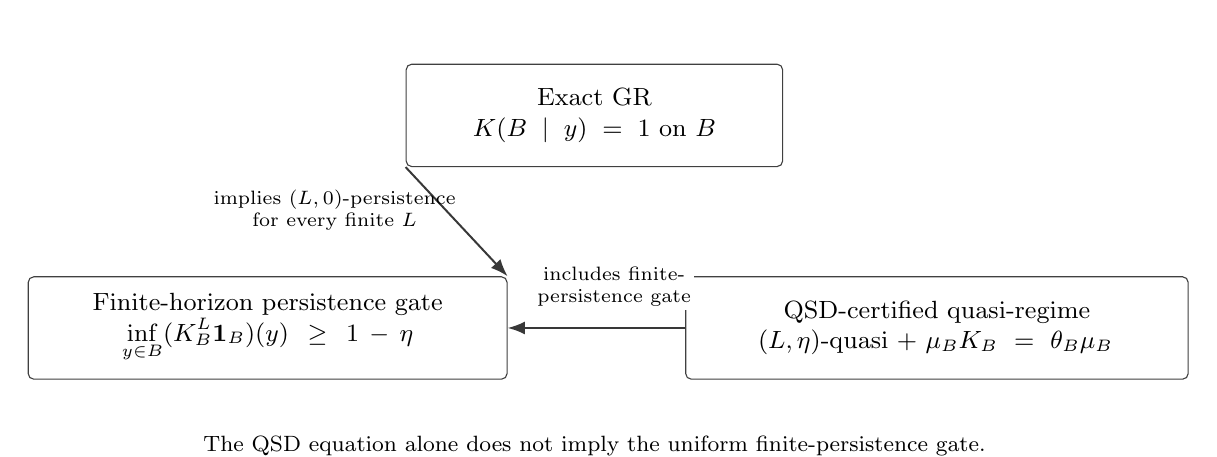
\begin{tikzpicture}[>=Latex,
  box/.style={draw=black!75,rounded corners=2pt,fill=white,align=center,minimum height=13mm,inner sep=4pt,font=\small},
  arr/.style={->,line width=.72pt,draw=black!78}]
\node[box, text width=45mm] (exact) at (0,1.55) {Exact GR\\$K(B\mid y)=1$ on $B$};
\node[box, text width=58mm] (finite) at (-4.15,-1.15) {Finite-horizon persistence gate\\$\displaystyle \inf_{y\in B}(K_B^L\mathbf 1_B)(y)\ge 1-\eta$};
\node[box, text width=61mm] (qsd) at (4.35,-1.15) {QSD-certified quasi-regime\\$(L,\eta)$-quasi $+\ \mu_BK_B=\theta_B\mu_B$};
\draw[arr] (exact.south west) -- (finite.north east);
\node[font=\scriptsize,align=center] at (-3.3,0.35) {implies $(L,0)$-persistence\\for every finite $L$};
\draw[arr] (qsd.west) -- (finite.east);
\node[font=\scriptsize,align=center,fill=white,inner sep=1.2pt] at (0.25,-0.63) {includes finite-\\persistence gate};
\node[font=\footnotesize,align=center] at (0,-2.65) {The QSD equation alone does not imply the uniform finite-persistence gate.};
\end{tikzpicture}
\caption{Persistence implications and QSD certification. Exact GR implies $(L,0)$-persistence at every finite horizon. A QSD-certified quasi-regime separately includes the finite-persistence gate and an eigenmeasure certificate; the QSD equation alone does not establish the uniform gate.}
\label{fig:persistence-hierarchy}
\end{figure}

\subsection{4.5 Regime locus}\label{regime-locus}

Because Y is typed, a GR can be classified by locus without changing the
underlying mathematics. A world-locus regime has \(B=S\times{}B_X\) and
a descriptor \(h=h_X\circ{}\operatorname{pr}_X\). A strategic-locus
regime has \(B=B_S\times{}X\) and \(h=h_S\circ{}\operatorname{pr}_S\). A
coupled regime uses a genuinely joint region or descriptor. This typing
is semantic information that is discarded by the enlarged-state
reduction but can matter for interpretation and interventions. The framework retains that semantic declaration operational in confirmatory PR
analysis through the relevance map introduced next: a world-locus claim
will normally project away representation-only strategic coordinates,
whereas a strategic or coupled claim may explicitly retain them.

\section{5. Permansson Regimes and Typed
Constitution}\label{permansson-regimes-and-typed-constitution}

\subsection{5.1 Why constitution is separate from
persistence}\label{why-constitution-is-separate-from-persistence}

A process can satisfy a GR specification for reasons that are exogenous
to the strategic generator. A favorable resource trend, an absorbing
world state, or a structural transition mechanism may create the
declared regime even if strategic behavior is irrelevant. Permansson
classification therefore adds an intervention-relative test: a strategic
component is constitutive only if a fixed admissible intervention on
that component changes a predeclared defining regime property while the
declared non-intervened primitives are held fixed.

\subsection{5.2 Regime-property maps}\label{regime-property-maps}

Fix a GR specification \(\Sigma\). Let \(Z_\psi\) be a metric space with
metric \(d_\psi\), and let

\begin{equation}
\psi:\Delta(\Omega)\longrightarrow Z_\psi.
\tag{14}\label{eq:14}
\end{equation}

be a predeclared regime-property map on admissible state-path laws. No
measurability assumption on \(\psi\) is needed for the pointwise
constitutive definitions (15)-(16); when an application treats estimated
or random path laws as random elements and then integrates, optimizes,
or otherwise randomizes \(\psi\), the corresponding measurability or
regularity must be imposed explicitly. The dependence of \(\psi\) on the
frozen descriptor and specification may be suppressed in notation.
Examples include exact persistence status, long-run growth class,
limiting composition, occupation mass on a target subset, strategic-mode
preservation, or a vector of such properties. For confirmatory PR
analysis, also freeze a Borel relevance map \(g:Y\to{}G\) into a
declared standard-Borel regime-observation space G. The map must be rich
enough to represent the baseline regime observables: \(B=g^{-1}(B_G)\)
for some Borel \(B_G\subseteq{}G\) and \(h=h_G\circ{}g\) for some Borel
\(h_G:G\to{}H\). Writing \(g^\infty\) for the coordinatewise path map,
\(\psi\) is g-grounded when there exists a predeclared map \(\psi_G\) on
path laws over G such that \(\psi(\mu)=\psi_G((g^\infty)_{\push}\mu)\)
for every admissible baseline or intervened path law. Thus the
constitutive comparison may use only state information explicitly
declared by g. If a claimed property depends on realized actions, a
sufficient action-mode record must be included in S and in g before the
specification is frozen. For a confirmatory PR claim, the semantic
counterfactual pipeline is frozen jointly before the counterfactual
outcome is evaluated, even though the GR gate may be checked first. The
frozen pipeline includes g, \(\psi\), \(B_1\), the component grammar,
the intervention protocol J, and any hard structural target/transport
conventions used to define that intervention. If the pipeline is
selected from data rather than predeclared, confirmatory use requires a
valid held-out or selection-adjusted procedure that covers the search.
The broad \(\mathrm{PR}_{\mathrm{general}}\) class remains
mathematically available without this extra relevance restriction;
grounded status is the confirmatory subclass used to exclude undeclared
representation padding.

Confirmatory applications should also conduct a relevance-map audit. The
audit should justify the substantive information retained by g; verify
that B, h, and \(\psi\) factor through g as claimed; search strict
coarsenings when feasible; report non-uniqueness when several
incomparable sufficient relevance maps exist; and rerun the
classification under defensible alternatives when the semantic choice is
not unique. A coordinate is not substantively relevant merely because
retaining it increases \(B_1\) diversity or predictive fit. The
framework does not assume that one uniquely minimal or canonical
relevance map always exists.

\subsection{5.3 Admissible typed
interventions}\label{admissible-typed-interventions}

Interventions are typed by the object they modify.

Formally, fix the ambient canonical environment
\((S,X,A,A(\cdot{}),\alpha,P,U)\). An admissible typed intervention J is
a predeclared map that returns replacement kernel(s) on the same
declared measurable spaces, satisfies the relevant measurability and
feasibility conditions, and states which elements of the environment are
held fixed. The label k or \(\ell\) identifies the predeclared target
component; constitution is always relative to this intervention protocol
rather than to an intrinsic decomposition of a kernel into unnamed
parts.

\begin{itemize}
\item
  Action-selection intervention \(J_k^\alpha\): replaces a predeclared
  component k of \(\alpha\) with a feasible measurable rule \(\alpha'\)
  while holding U, P, the feasible-action correspondence, and all other
  declared primitives fixed.
\item
  Strategic-update intervention \(J_k^U\): replaces a predeclared
  component k of U with a measurable update kernel \(U'\) while holding
  \(\alpha\) and P fixed.
\item
  Strategic-generator intervention \(J_k^{\mathfrak G}\): changes a
  declared component of \(\alpha\), U, or both, with all unaffected
  components listed explicitly.
\item
  World-transition intervention \(J_\ell^P\): replaces a declared
  component of P while holding \(\mathfrak G\) fixed.
\item
  Institutional or structural intervention: changes feasibility,
  information, admission rules, or other model primitives. If the
  original generator becomes infeasible, the protocol must declare a
  replacement admissible behavior rule. Such an intervention is not
  silently reclassified as a generator intervention.
\end{itemize}

Two admissibility levels must be kept separate. Formal admissibility is
the kernel-level requirement above: the intervention is well typed,
measurable, feasible, and explicit about the objects held fixed.
Confirmatory empirical admissibility is stronger. It additionally
requires a defensible claim that the held-fixed mechanisms would remain
invariant under the intervention over every state/action row that
becomes intervention-reachable.

For confirmatory empirical use, fix the predeclared hard structural
compatibility relations and let T denote the declared target. Let T*
denote the closure of T under those hard relations. If preserving a hard
identity forces another component to move, the intervention must
expand/retype its target or be declared inadmissible under that
structural specification. Hard identities must be distinguished from
soft fitted parameter ties or convenient parametric families; leaving an
estimated family is not by itself an admissibility failure.

Causal modularity and support are empirical claim requirements rather
than additions to the formal intervention definition. Evidence for a
held-fixed mechanism may come from randomized variation, justified
sufficient-state adjustment, structural equations, natural experiments,
engineering or institutional mechanism knowledge, or another defensible
causal design. Full observational action support alone is not
sufficient. If an intervention reaches unsupported rows that matter to
\(\psi\), or if the stability of the held-fixed mechanism is unresolved,
the formal counterfactual may remain mathematically defined while the
application records identification status
\texttt{STRUCTURALLY\_UNRESOLVED}; statistical status, if applicable, is
reported separately.

The intervened strategic generator need not be an equilibrium or a best
response. The purpose of the intervention is diagnostic constitution,
not post-intervention equilibrium certification. A date-indexed
intervention is admissible in the stationary canonical core only after a
clock variable has been included in S; equivalently it belongs to the
nonautonomous extension. Section 6 uses the clock-state construction to
embed the full Paper-I intervention grammar.

\subsection{5.4 Constitutive components}\label{constitutive-components}

Let \(B_1\subseteq{}B_0\) be a predeclared Borel set containing at least
two states with distinct baseline path laws. Let \(J_k^{\mathfrak G}\)
be an admissible strategic-generator intervention. A strategic-generator
component k is \((\psi,J_k^{\mathfrak G},B_1)\)-constitutive if

\begin{equation}
\psi\!\left(P_y^{\mathfrak G,P}\right)\ne \psi\!\left(P_y^{J_k^{\mathfrak G}(\mathfrak G),P}\right)\qquad\text{for every }y\in B_1.
\tag{15}\label{eq:15}
\end{equation}

It is uniformly constitutive if there exists \(\delta_\psi>0\) such that

\begin{equation}
\inf_{y\in B_1} d_\psi\!\left(\psi(P_y^{\mathfrak G,P}),\psi(P_y^{J_k^{\mathfrak G}(\mathfrak G),P})\right)\ge\delta_\psi.
\tag{16}\label{eq:16}
\end{equation}

For quantitative analysis define the pointwise constitutive effect profile and its uniform margin by

\begin{equation}
\Delta_{\psi,J}(y)=d_\psi\!\left(\psi(P_y),\psi(P_y^J)\right),\qquad
\kappa_{\psi,J}(B_1)=\inf_{y\in B_1}\Delta_{\psi,J}(y).
\tag{16a}\label{eq:16a}
\end{equation}

Thus pointwise constitution requires \(\Delta_{\psi,J}(y)>0\) for every \(y\in B_1\), while uniform constitution is equivalent to \(\kappa_{\psi,J}(B_1)>0\). Pointwise constitution alone does not imply a positive uniform margin.


A component \(\ell\) of P is structurally constitutive under an
admissible \(J_\ell^P\) when the analogous property holds with
\(\mathfrak G\) fixed. Strategic and structural constitution can
coexist. Structural constitution by itself does not make the regime a
Permansson regime, preserving the naming logic of the earlier EGR paper.

Definition 5.1 (Generalized Permansson Regime). An Exact GR
\(R=(\mathfrak G,P,B,B_0,h,\nu,\mathfrak c)\) is a generalized
Permansson Regime relative to \((\psi,J_k^{\mathfrak G},B_1)\) if at
least one predeclared component k of the strategic generator is
constitutive of a defining regime property \(\psi\) under the admissible
intervention \(J_k^{\mathfrak G}\) on the predeclared set \(B_1\).
Uniform PR status uses condition (16). A generalized PR is grounded
relative to a frozen relevance map g when B and h factor through g as
specified in Section 5.2 and \(\psi\) is g-grounded. The formal grounded
subclass used as a prerequisite for confirmatory applications requires
both a descriptor-nondegenerate Exact-GR baseline and grounded PR
status; denote this subclass \(\mathrm{PR}_g\) when a compact label is
useful. Empirical confirmation additionally requires the
application-level certificate of Sections 10.5-10.7.

PR status is therefore relative to a baseline model, regime
specification, property map, intervention protocol, and initial-state
set; grounded confirmatory status is additionally relative to the frozen
relevance map g. It is not an intrinsic label attached to
\(K_{\mathfrak G,P}\) alone. The distinction matters under state
augmentation: \(\mathrm{PR}_{\mathrm{general}}\) deliberately permits
any predeclared typed-state property, whereas \(\mathrm{PR}_g\) refuses
to let a coordinate omitted from g create a confirmatory constitutive
claim.

Component attribution is grammar-relative. A compound block may be
constitutive even when no singleton is; a singleton effect may disappear
when components are merged; and several incomparable constitutive blocks
may coexist. Confirmatory applications should therefore freeze the
component grammar and target before inspection of the counterfactual,
record whether the target is atomic, compound, or jointly defined, and
test substantively meaningful coarsenings or refinements when
attribution matters. Under reparameterization, interventions must be
transported by their substantive meaning rather than matched by raw
coordinate labels. Constitution under a frozen intervention is a
stronger claim than unique attribution to one intrinsically privileged
component.


\subsubsection{5.4.1 Quantitative perturbation certification}\label{quantitative-perturbation-certification}

The margin in (16a) permits a general robustness statement that is independent of how the baseline and intervention error bounds were obtained. Let \(\widetilde P_y\) and \(\widetilde P_y^J\) denote perturbed or approximated baseline and intervention path laws evaluated by the same frozen property map \(\psi\).

\textbf{Proposition 5.2 (Two-sided constitutive-margin perturbation bound).} Suppose, uniformly for \(y\in B_1\),

\begin{equation}
d_\psi\!\left(\psi(P_y),\psi(\widetilde P_y)\right)\le\varepsilon_0,
\qquad
d_\psi\!\left(\psi(P_y^J),\psi(\widetilde P_y^J)\right)\le\varepsilon_J.
\tag{16b}\label{eq:16b}
\end{equation}

Then for every \(y\in B_1\),

\begin{equation}
\left|\Delta_{\psi,J}(y)-\widetilde\Delta_{\psi,J}(y)\right|\le\varepsilon_0+\varepsilon_J,
\tag{16c}\label{eq:16c}
\end{equation}

and, writing \(\widetilde\kappa\) for the perturbed uniform margin on the same \(B_1\),

\begin{equation}
|\widetilde\kappa-\kappa|\le\varepsilon_0+\varepsilon_J,
\qquad
\widetilde\kappa\ge\kappa-\varepsilon_0-\varepsilon_J.
\tag{16d}\label{eq:16d}
\end{equation}

\emph{Proof.} For any four points \(a,b,\widetilde a,\widetilde b\) in a metric space, the triangle inequality and its reverse form imply
\[
|d(a,b)-d(\widetilde a,\widetilde b)|\le d(a,\widetilde a)+d(b,\widetilde b).
\]
Apply this with the baseline and intervention property outputs to obtain (16c). If two real-valued functions differ uniformly by at most e, their infima differ by at most e; applying this with \(e=\varepsilon_0+\varepsilon_J\) yields (16d). \hfill\textsc{q.e.d.}

\textbf{Corollary 5.3 (Robust PR certificate).} If \(\kappa_{\psi,J}(B_1)>\varepsilon_0+\varepsilon_J\), then \(\widetilde\kappa>0\) and uniform constitutive status survives the perturbation. Equality \(\kappa=\varepsilon_0+\varepsilon_J\) does not certify survival. This theorem is a bridge from property-output error to PR classification; it does not by itself provide \(\varepsilon_0\) or \(\varepsilon_J\).

\textbf{Proposition 5.4 (Finite-horizon kernel-to-path envelope).} Use the probability-distance convention \(\|\mu-\nu\|_{\mathrm{TV}}:=\sup_A|\mu(A)-\nu(A)|\). Let K and \(\widetilde K\) be Markov kernels on the same state space and let \(\varepsilon\in[0,1]\) satisfy
\[
\sup_y\|K(y,\cdot)-\widetilde K(y,\cdot)\|_{\mathrm{TV}}\le\varepsilon.
\]
From the same point initial state y, let \(P_y^{0:T}\) and \(\widetilde P_y^{0:T}\) denote the path laws through T transitions. Then

\begin{equation}
\|P_y^{0:T}-\widetilde P_y^{0:T}\|_{\mathrm{TV}}
\le 1-(1-\varepsilon)^T\le T\varepsilon.
\tag{16e}\label{eq:16e}
\end{equation}

\emph{Proof.} Couple the chains step by step. Conditional on agreement through time t, use a maximal coupling of \(K(Y_t,\cdot)\) and \(\widetilde K(Y_t,\cdot)\); the probability of remaining coupled for the next transition is at least \(1-\varepsilon\). Hence the probability of agreement through T transitions is at least \((1-\varepsilon)^T\). The coupling inequality gives the first bound; Bernoulli's inequality gives the second. \hfill\textsc{q.e.d.}

No infinite-horizon analogue is asserted without additional structure. Small one-step kernel perturbations can cause order-one changes in stationary or infinite-path behavior near loss of ergodicity, and discontinuous \(\psi\) can flip under arbitrarily small law perturbations. For long-run occupation laws, invariant laws, or QSDs, kernel-to-law
bounds are used only in subclasses satisfying the corresponding uniform-ergodic, contraction, spectral, or killed-process hypotheses (Mitrophanov, 2005; Rudolf and Wang, 2025).

\subsection{5.5 Protocol scope and negative
claims}\label{protocol-scope-and-negative-claims}

Definition 5.1 makes PR status relative to the frozen
property/intervention protocol \((\psi,J,B_1)\). Failure of one declared
intervention therefore establishes only nonconstitution under that
protocol; it is not a global statement that no strategically
constitutive intervention exists. For applications, use the label
\status{ROBUST_NONCONSTITUTIVE_UNDER_FROZEN_PROTOCOL} when a
declared protocol is excluded over the required state/model set. A
broader \status{NO_PR_IN_DECLARED_INTERVENTION_FAMILY} claim
requires exclusion of every member of a predeclared admissible
intervention family, or a theorem that rules the family out.

This protocol scope is especially important under partial
identification. A negative claim must quantify over the same
provenance-valid model set, \(B_1\), and declared intervention family
that define the application. Non-significance, failure to obtain a
uniform gap, or failure of one intervention does not by itself establish
global non-PR status.

\subsection{5.6 Regime equivalence}\label{regime-equivalence}

The regime layer supports several deliberately distinct equivalence
notions. For the cleanest comparison, let two GRs share a common
descriptor space H, descriptor h, convergence mode, and declared
comparison set \(I\subseteq{}Y\). Let
\(h^\infty:\Omega\to{}H^{\mathbb N_0}\) be the coordinatewise descriptor
map \(h^\infty((Y_t)_t)=(h(Y_t))_t\).

\begin{itemize}
\item
  Strong descriptor path-law equivalence:
  \((h^\infty)_{\push}P_y^{(1)}=(h^\infty)_{\push}P_y^{(2)}\) for every
  \(y\in{}I\).
\item
  Occupation equivalence: both satisfy the same declared persistence
  requirement and convergence mode and have the same limiting occupation
  law \(\nu\) on H.
\item
  Property equivalence: \(\psi(P_y^{(1)})=\psi(P_y^{(2)})\) for every y
  in the declared comparison set on which \(\psi\) is evaluated.
\item
  Constitutive equivalence relative to matched interventions
  \(J_1,J_2\): baseline property equivalence holds and
  \(\psi(P_y^{(1),J_1})=\psi(P_y^{(2),J_2})\) for every declared
  comparison state y; uniform constitutive equivalence additionally
  preserves the corresponding \(d_\psi\) gaps.
\end{itemize}

The last notion is strictly stronger than baseline dynamical
equivalence. This distinction is the main substantive reason to preserve
the strategic/world factorization after conceding the enlarged-state
reduction.

\section{6. Embedding the Equilibrium-Generated
Theory}\label{embedding-the-equilibrium-generated-theory}

\subsection{6.1 Paper-I EGR object}\label{paper-i-egr-object}

The earlier EGR core assumes a discounted stochastic game with a Polish
payoff-relevant state space X, finite feasible action sets, bounded
measurable stage payoffs, a measurable state-transition kernel P,
discount factors, and a selected measurable pure stationary
Markov-perfect equilibrium \(\pi^\ast\). The equilibrium induces
\(P^{\pi^\ast}(D\mid x)=P(D\mid x,\pi^\ast(x))\). An EGR is
\(R_E=(\pi^\ast,B,B_0,h,\nu,\mathfrak c)\) with ex ante non-triviality,
exact invariance of B under \(P^{\pi^\ast}\), and the declared
occupation-law convergence for every initial law supported on \(B_0\)
(Hermansson, 2026a).

\subsection{6.2 Canonical embedding}\label{canonical-embedding}

For the fully conservative embedding, let A be the finite Paper-I joint
action space, adjoin a symbol \(\bot\notin{}A\), and define the
strategic state \(S_E=\mathbb N_0\times{}(A\cup{}\{\bot\})\) with the
discrete topology. The coordinate \(s_t=(t,a_{t-1})\) records the clock
and the previously realized joint action, with \(a_{-1}=\bot\). Let

\begin{equation}
\begin{aligned}\alpha^{\pi^\ast}(da\mid(t,\bar a),x)&=\delta_{\pi^\ast(x)}(da),\\[2pt]U^{\mathrm{rec}}(ds'\mid(t,\bar a),x,a,x')&=\delta_{(t+1,a)}(ds').\end{aligned}
\tag{17}\label{eq:17}
\end{equation}

Retain the original world-transition law by setting
\(P_E(dx'\mid (t,\bar a),x,a)=P(dx'\mid x,a)\). Let
\(\iota_0(x)=((0,\bot),x)\), lift the regime region to
\(\widetilde B=S_E\times{}B\), and lift the initial basin to
\(\widetilde B_0=\iota_0(B_0)\). The action record makes every realized
\(A_t\) measurable from the next strategic coordinate \(S_{t+1}\); the
clock makes date-indexed Paper-I interventions state-indexed in the
enlarged model.

On embedded paths define the measurable decoding map D by
\(D(((t,\bar a_t),x_t)_{t\ge{}0})=((x_t)_{t\ge{}0},(a_t)_{t\ge{}0})\),
with \(a_t=\bar a_{t+1}\). On the null/off-support set of paths that do
not satisfy the recording relation, extend D arbitrarily. Thus both the
Paper-I world path and the realized action sequence are recoverable from
the embedded state path.

\begin{equation}
\begin{aligned}K_{\mathfrak G^{\pi^\ast},P_E}(S_E\times D\mid(t,\bar a),x)&=P(D\mid x,\pi^\ast(x))\\&=P^{\pi^\ast}(D\mid x).\end{aligned}
\tag{18}\label{eq:18}
\end{equation}

Because Paper I defines h only on B, choose any \(h_0\in{}H\) and the
Borel extension \ensuremath{\bar h}(x)=h(x) for \(x\in{}B\) and \(\bar h(x)=h_0\)
otherwise; define \(\widetilde h((t,\bar a),x)=\bar h(x)\). If the
measure branch of Paper-I non-triviality is used, lift the reference
measure by \(\widetilde m=(\iota_0)_{\push}m\). If the interior branch
is used, \ensuremath{\widetilde B} has nonempty interior whenever B does because \(S_E\) is
discrete. For grounded confirmatory transport, the default relevance map
is \(\widetilde g((t,\bar a),x)=x\); if a Paper-I property explicitly
depends on the recorded action or another transported mode, enlarge \ensuremath{\widetilde g} ex
ante to include the corresponding sufficient record.

\textbf{Theorem 6.1 (EGR embedding).} The lifted object
\(\iota(R_E)=(\mathfrak G^{\pi^\ast},P_E,\widetilde B,\widetilde B_0,\widetilde h,\nu,\mathfrak c)\)
is an Exact GR if and only if \(R_E\) is an EGR in the earlier theory.
Under projection \(\operatorname{pr}_X:S_E\times{}X\to{}X\), the
baseline world-state path laws, exact persistence status, descriptor
process on the baseline region, limiting occupation law, and convergence
mode are identical.

Proof. Equation (18) gives the Paper-I equilibrium-induced kernel as the
X-marginal of the embedded transition. Starting from any law supported
on \(\widetilde B_0\), induction shows that the X-coordinate has exactly
the Paper-I path law and that \(S_t=(t,A_{t-1})\) records the realized
action history. Exact invariance of B implies exact invariance of \ensuremath{\widetilde B}, and
conversely projection of any embedded path in \ensuremath{\widetilde B} lies in B. Since \ensuremath{\widetilde h}=h on
B, the empirical descriptor measures are identical along all baseline
paths. The lifted non-triviality conditions follow from the
constructions of \ensuremath{\widetilde B}, \(\widetilde B_0\) and \ensuremath{\widetilde m}. Moreover, the
basin-reachable descriptor-law family is identical under projection, so
descriptor-nondegenerate Paper-I applications remain
descriptor-nondegenerate after embedding. The same projection also
transports the optional forward-richness diagnostic. \hfill\textsc{q.e.d.}

\subsection{6.3 Conservative recovery of the original Permansson
regime}\label{conservative-recovery-of-the-original-permansson-regime}

In Paper I, a policy intervention \(J_k^\pi\) may replace a predeclared
policy component on declared states or dates. Let \(C_I\) denote the
class of admissible Paper-I constitutive property/intervention
protocols, and let \(\iota_{\push}C_I\) denote the protocols transported
into the canonical strategic-world environment by the construction
below. Define \(\mathrm{PR}_{\iota}\) as generalized PR status evaluated
only relative to protocols in \(\iota_{\push}C_I\); when comparing with
Paper I, restrict this status to embedded EGR objects. For
\(J_k^\pi\in{}C_I\), let \(\rho_t^J(x)\) denote the resulting feasible
joint action rule, equal to \(\pi^\ast(x)\) off the intervention set.
Map it to the action-selection intervention
\(\alpha^J(da\mid (t,\bar a),x)=\delta_{\rho_t^J(x)}(da)\), while
keeping \(U^{\mathrm{rec}}\) and \(P_E\) fixed. Thus date-indexed
interventions are represented without changing the canonical Markov
form, and the strategic state records the realized intervention action
one step later.

Theorem 6.2 (Conservative Permansson extension). Let \(R_E\) be an EGR
and let \((\psi_I,J_k^\pi,B_1)\) be an admissible Paper-I constitutive
protocol whose property functional is well defined on both the baseline
and intervened laws under a frozen descriptor convention. If an
intervention may leave B and \(\psi_I\) evaluates h after exit, include
a predeclared Borel extension \ensuremath{\bar h} in that convention. Define the
transported property map on embedded path laws by
\(\widetilde\psi(\mu)=\psi_I((\operatorname{pr}_X^\infty)_{\push}\mu,\bar h)\),
or by the corresponding measurable decode \(D_{\push}\mu\) when the
Paper-I protocol explicitly includes recorded actions. For grounded
confirmatory transport, take \(\widetilde g((t,\bar a),x)=x\) for
world-path properties and enlarge \ensuremath{\widetilde g} ex ante to \((x,\bar a)\), the
clock, or another sufficient transported record only when the Paper-I
property actually uses that information. Then \(R_E\) is a Permansson
regime under the Paper-I definition if and only if its embedding
\(\iota(R_E)\) is a generalized Permansson regime relative to
\((\widetilde\psi,J_k^\alpha,\widetilde B_1)\), where
\(\widetilde B_1=\iota_0(B_1)\); whenever the transported
\(\widetilde\psi\) is \ensuremath{\widetilde g}-grounded, grounded status is preserved as well.

Proof. Baseline world-state path laws coincide by Theorem 6.1. Under the
mapped intervention, \(\alpha^J\) chooses exactly the Paper-I intervened
action at each declared date/state, \(P_E\) remains the original
transition law, and \(U^{\mathrm{rec}}\) merely records the realized
action. Hence the projected state path and, where used, the decoded
action path coincide with the Paper-I counterfactual execution. By
construction of \(\widetilde\psi\) and the common frozen descriptor
convention, baseline and intervention \(\psi\)-values are identical to
their Paper-I counterparts for every \(y\in{}B_1\), as are the
corresponding \(d_\psi\) distances. When grounded transport is
requested, \ensuremath{\widetilde g} contains exactly the state/action record used by the
Paper-I property, so \(\widetilde\psi\) factors through
\((\widetilde g^\infty)_{\push}\) by construction. Therefore pointwise,
uniform, and grounded constitution are preserved in both directions.
\hfill\textsc{q.e.d.}

Theorems 6.1 and 6.2 establish the conservative hierarchy after
identifying Paper-I objects with their images under \(\iota\):
\(\iota(\mathrm{EGR})\subseteq{}\mathrm{GR}\),
\(\mathrm{PR}_{\iota}\subseteq{}\mathrm{PR}_{\mathrm{general}}\subseteq{}\mathrm{GR}\),
and
\(\iota(\mathrm{PR}_{\mathrm{old}})=\iota(\mathrm{EGR})\cap{}\mathrm{PR}_{\iota}\).
No equality is asserted with the unrestricted intersection
\(\iota(\mathrm{EGR})\cap{}\mathrm{PR}_{\mathrm{general}}\). The latter
may contain additional generalized constitutive classifications that act
on strategic-update or auxiliary representation components absent from
the Paper-I policy grammar. The grounded confirmatory layer does not alter
this broad hierarchy:
\(\mathrm{PR}_g\subseteq{}\mathrm{PR}_{\mathrm{general}}\), and
transported Paper-I protocols are grounded whenever their relevance map
is frozen to the world/action information actually used by the original
property.

\section{7. Representation, Identification, and Constitutive
Equivalence}\label{representation-identification-and-constitutive-equivalence}

\subsection{7.1 Baseline representation
invariance}\label{baseline-representation-invariance}

\textbf{Proposition 7.1 (Baseline representation invariance).} Let two
well-posed canonical factorizations \((\mathfrak G_1,P_1)\) and
\((\mathfrak G_2,P_2)\) be defined on the same joint state space Y and
satisfy \(K_{\mathfrak G_1,P_1}=K_{\mathfrak G_2,P_2}\). Suppose they
use the same frozen regime specification \(\Sigma\) and the same
reference measure m whenever the measure branch of Assumption 4.1 is
invoked. Then \(R_1\) is an Exact GR if and only if \(R_2\) is an Exact
GR, with identical persistence and occupation-law classification.

\emph{Proof.} The exact-GR definition depends on the baseline model only
through the induced kernel and its path laws, together with the common
frozen specification. Equality of K gives equality of all
finite-dimensional distributions for common initial laws and hence
equality of path laws. Exact invariance and descriptor occupation
convergence therefore coincide. \hfill\textsc{q.e.d.}

\subsection{7.2 Factorization is not identified by the joint
process}\label{factorization-is-not-identified-by-the-joint-process}

\textbf{Theorem 7.2 (Factorization non-identification).} Equality of
induced joint kernels does not imply equality of the strategic generator
or world-transition kernel. In general,
\(K_{\mathfrak G_1,P_1}=K_{\mathfrak G_2,P_2}\) does not imply
\(\mathfrak G_1=\mathfrak G_2\) or \(P_1=P_2\).

Proof. Consider \(S=\{\star\}\), \(X=\{0,1\}\), \(A=\{0,1\}\), and
trivial U. In Factorization A, let
\(\alpha_A(\cdot{}\mid \star,x)=\delta_0\) and
\(P_A(\cdot{}\mid \star,x,a)=(1/2)\delta_0+(1/2)\delta_1\) for every
x,a. In Factorization B, let
\(\alpha_B(\cdot{}\mid \star,x)=(1/2)\delta_0+(1/2)\delta_1\) and
\(P_B(\cdot{}\mid \star,x,a)=\delta_a\). Under both factorizations the
next world state is Bernoulli(1/2), independent of the current state, so
the induced K is identical. Yet \(\alpha_A\ne{}\alpha_B\) and
\(P_A\ne{}P_B\). \hfill\textsc{q.e.d.}

The theorem has an immediate epistemic implication: the strategic/world
decomposition is a structural modeling claim. Observational equality of
the enlarged-state process is insufficient to identify which part of the
observed transition came from behavior selection and which part came
from world response.

\subsection{7.3 Baseline dynamical equivalence need not imply
constitutive
equivalence}\label{baseline-dynamical-equivalence-need-not-imply-constitutive-equivalence}

\begin{figure}[htbp]
\centering
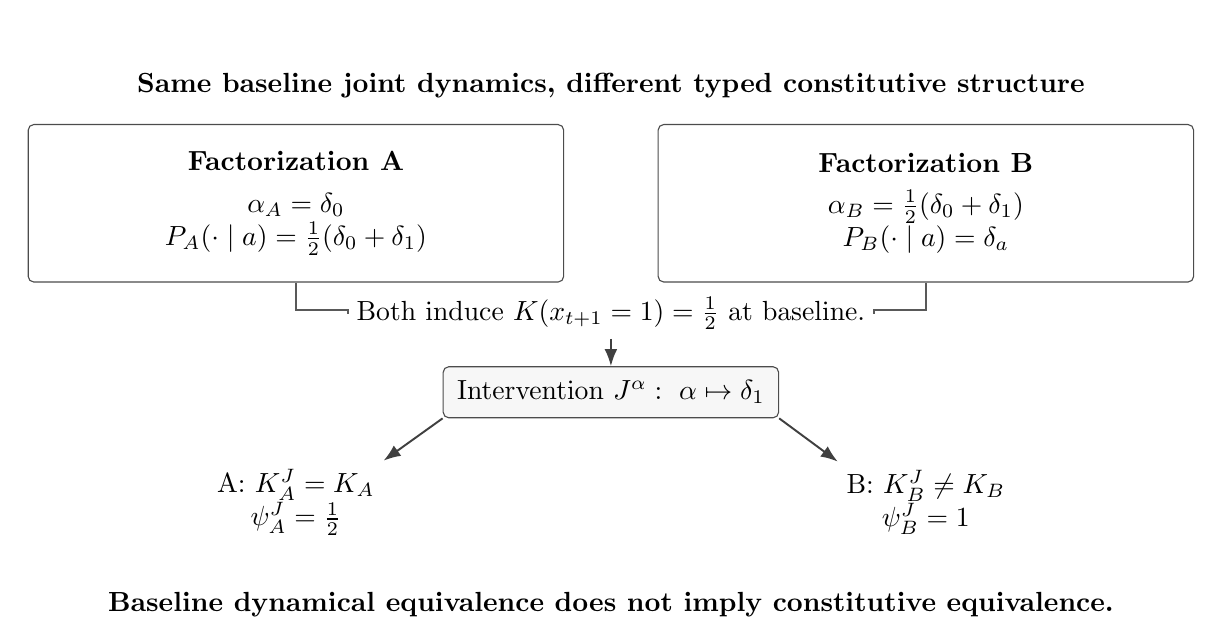
\begin{tikzpicture}[
  >=Latex,
  panel/.style={draw=black!70, rounded corners=2pt, fill=white, align=center, inner sep=5pt, minimum width=68mm, minimum height=20mm},
  mid/.style={draw=black!70, rounded corners=2pt, fill=black!3, align=center, inner sep=5pt},
  arr/.style={->,line width=.7pt,draw=black!75}
]
\node[font=\bfseries] at (0,3.55) {Same baseline joint dynamics, different typed constitutive structure};
\node[panel] (A) at (-4.0,2.05) {\textbf{Factorization A}\\[3pt]$\alpha_A=\delta_0$\\$P_A(\cdot\mid a)=\tfrac12(\delta_0+\delta_1)$};
\node[panel] (B) at (4.0,2.05) {\textbf{Factorization B}\\[3pt]$\alpha_B=\tfrac12(\delta_0+\delta_1)$\\$P_B(\cdot\mid a)=\delta_a$};
\node[fill=white,inner sep=3pt] (base) at (0,.65) {Both induce $K(x_{t+1}=1)=\tfrac12$ at baseline.};
\node[mid] (J) at (0,-.35) {Intervention $J^\alpha:\ \alpha\mapsto\delta_1$};
\node[fill=white,inner sep=3pt,align=center] (AO) at (-4.0,-1.75) {A: $K_A^J=K_A$\\$\psi_A^J=\tfrac12$};
\node[fill=white,inner sep=3pt,align=center] (BO) at (4.0,-1.75) {B: $K_B^J\ne K_B$\\$\psi_B^J=1$};
\draw[line width=.7pt,draw=black!65] (A.south) -- ++(0,-.35) -| (base.west);
\draw[line width=.7pt,draw=black!65] (B.south) -- ++(0,-.35) -| (base.east);
\draw[arr] (base) -- (J);
\draw[arr] (J.south west) -- (AO.north east);
\draw[arr] (J.south east) -- (BO.north west);
\node[font=\bfseries] at (0,-3.05) {Baseline dynamical equivalence does not imply constitutive equivalence.};
\end{tikzpicture}
\caption{Counterexample behind Theorem 7.3. Two factorizations induce the same baseline Markov kernel but react differently to the same action-selection intervention.}
\label{fig:counterexample}
\end{figure}

\textbf{Theorem 7.3 (Constitutive non-invariance under baseline
equivalence).} There exist two factorizations with the same baseline
joint kernel and the same Exact GR classification such that a matched
action-selection intervention is non-constitutive in one factorization
and uniformly constitutive in the other.

\emph{Proof.} Use the two factorizations from Theorem 7.2 and identify the joint state with $Y=\{\star\}\times\{0,1\}$. Let $B=B_0=Y$, let $h(\star,x)=x$ on all of $Y$, let $H=\{0,1\}$, let $\nu=\tfrac12\delta_0+\tfrac12\delta_1$, let $B_1=B_0$, use counting measure as the reference measure, and take $d_\psi$ to be absolute distance on $Z_\psi=[0,1]$. The baseline kernel is i.i.d. Bernoulli$(1/2)$ on the world coordinate after the initial state, so $B$ is exactly invariant and the empirical occupation measure converges almost surely to $\nu$ by the strong law. Define the total property map $\psi:\Delta(\Omega)\to[0,1]$ by
\[
\psi(\mu)=\limsup_{T\to\infty}\frac1T\sum_{t=0}^{T-1}\int x_t\,d\mu,
\]
where $x_t$ is the world coordinate at time $t$. On the product path space over a finite discrete state space, each finite-$T$ cylinder functional is continuous; therefore $\psi$, as a limsup of continuous real-valued functionals, is Borel. Baseline $\psi=1/2$ from either initial state. Apply the matched action-selection intervention $J$ setting $\alpha(\cdot\mid\star,x)=\delta_1$. In Factorization A, $P_A$ ignores the action, so $K$ and $\psi$ remain unchanged; the action-selection component is not constitutive. In Factorization B, $P_B$ sets $x'=a$, so after the intervention the process reaches $x=1$ after at most one transition and $\psi=1$. The $d_\psi$-gap is therefore $1/2$ uniformly over $B_1$. Hence the same baseline $K$ supports different constitutive classifications. \hfill\textsc{q.e.d.}

\subsection{7.4 Intervention-compatible
invariance}\label{intervention-compatible-invariance}

The previous theorem does not make constitutive classification
arbitrary. It identifies the extra information that must be fixed. Two
factorizations are intervention-compatible relative to \(J_1\) and
\(J_2\) when they have the same baseline K and their matched
interventions also induce the same post-intervention kernel.

Proposition 7.4 (Intervention-compatible invariance). If \(K_1=K_2\) and
\(K_1^{J_1}=K_2^{J_2}\), and the same \(\psi\), \(B_1\), descriptor
specification, and grounded relevance map are used, then a component is
constitutive under \(J_1\) in model 1 if and only if the matched
component is constitutive under \(J_2\) in model 2. The same holds for
uniform constitution with the same \(d_\psi\) distance.

\emph{Proof.} Baseline path laws coincide and post-intervention path
laws coincide. The defining inequalities in (15) and (16) are therefore
identical. \hfill\textsc{q.e.d.}

This result provides the appropriate representation-invariance standard
for PR claims. Baseline K equivalence is sufficient for GR equivalence.
PR equivalence additionally requires agreement on the counterfactual
intervention semantics; grounded confirmatory equivalence also requires
agreement on the declared regime-observation map.


\subsubsection{7.4.1 Frozen intervention-family signatures}\label{frozen-intervention-family-signatures}

Let \(\mathcal J\) be a predeclared intervention family. For a model M write its frozen intervention signature as

\begin{equation}
\operatorname{Sig}_{\mathcal J}(M)=\left(K_M,(K_M^J)_{J\in\mathcal J}\right).
\tag{18a}\label{eq:18a}
\end{equation}

\textbf{Proposition 7.4a (Intervention-family invariance).}\par\noindent Let \(M_1\) and \(M_2\) use the same state space, frozen regime/property/relevance semantics, and comparison set \(B_1\). Suppose there is a predeclared target/type-grammar-preserving bijection \(\phi:\mathcal J_1\to\mathcal J_2\) satisfying
\[
K_1=K_2,\qquad K_1^J=K_2^{\phi(J)}\quad\text{for every }J\in\mathcal J_1.
\]
Then every matched pointwise constitutive classification, uniform margin, and protocol-scoped negative classification over that family is identical in the two models.

\emph{Proof.} Equality of each baseline kernel and each matched post-intervention kernel gives equality of the corresponding point-initialized path laws. Applying the same \(\psi\) and \(d_\psi\) therefore gives identical \(\Delta_{\psi,J}(y)\) for every y and J, hence identical infima and classifications. \hfill\textsc{q.e.d.}

The family and the label matching must be frozen ex ante. The bijection preserves the declared intervention target/type grammar (for example, an action-selection intervention is matched to the corresponding action-selection intervention), rather than merely pairing equal induced kernels after inspection. Equality for the baseline and only a selected subset of intervention labels does not justify an equivalence claim for omitted labels; a post-hoc choice of the matching family is a semantic selection step rather than a representation theorem.

\subsubsection{7.4.2 Intervention-compatible state quotients}\label{intervention-compatible-state-quotients}

The next result gives sufficient, not necessary, conditions under which state compression preserves the regime layer. It is intentionally stronger than ordinary baseline lumpability because PR status depends on counterfactual kernels and frozen semantics.

\textbf{Theorem 7.4b (Intervention-compatible quotient preservation).} Let M and \(\bar M\) be well-posed canonical strategic-world models of Section 3 with joint Polish state spaces \(Y=S\times X\) and \(\bar Y=\bar S\times\bar X\). Let \(q_S:S\to\bar S\) and \(q_X:X\to\bar X\) be measurable surjections and let the state compression be the type-respecting product map \(q=q_S\times q_X:Y\to\bar Y\). Let \(\mathcal J\) and \(\bar{\mathcal J}\) be frozen typed intervention families with a predeclared target/type-grammar-preserving bijection \(\phi:\mathcal J\to\bar{\mathcal J}\); treat the baseline as label 0 and set \(\phi(0)=0\). Write \(K^J\) and \(\bar K^{\phi(J)}\) for the induced baseline or post-intervention kernels of the two canonical models. Suppose:
\begin{enumerate}[label=(\roman*),leftmargin=2.2em]
\item for every \(J\in\{0\}\cup\mathcal J\),
\[
K^J(q^{-1}(C)\mid y)=\bar K^{\phi(J)}(C\mid q(y))
\]
for every y and Borel \(C\subseteq\bar Y\);
\item \(B=q^{-1}(\bar B)\), \(B_0=q^{-1}(\bar B_0)\), and both the original and quotient specifications independently satisfy Assumption 4.1;
\item \(h=\bar h\circ q\) and the same descriptor target law \(\nu\) and convergence mode are used;
\item \(B_1=q^{-1}(\bar B_1)\), and \(B_1\) and \(\bar B_1\) independently satisfy the comparison-set admissibility/non-triviality requirement of Section 5.4;
\item \(\psi\) and \(\bar\psi\) take values in the same metric property space \((Z_\psi,d_\psi)\), and on all baseline and frozen-intervention path laws used in the comparison,
\[
\psi(P)=\bar\psi\!\left((q^\infty)_{\push}P\right);
\]
for grounded claims, \(g=\bar g\circ q\); and
\item every probability law on \(\bar B_0\) considered by the quotient specification has an admissible lift \(\lambda\) on \(B_0\) with \(q_{\push}\lambda=\bar\lambda\).
\end{enumerate}
Then Exact-GR status is preserved between M and \(\bar M\), and for every \(J\in\mathcal J\) the corresponding pointwise and uniform PR classifications and margins are preserved under the matched intervention \(\phi(J)\). The theorem assumes, rather than reconstructs, the canonical strategic/world factorization and typed intervention/component grammar of the quotient model; the product form of q prevents the quotient itself from relabelling strategic coordinates as world coordinates or conversely.

\emph{Proof.} The kernel-intertwining identity in (i) implies by induction on cylinder sets that \((q^\infty)_{\push}P_y^{K^J}=P_{q(y)}^{\bar K^{\phi(J)}}\) for every point initial state y and every J, including the baseline. Because \(B=q^{-1}(\bar B)\), exact invariance is equivalent statewise under q. Because \(h=\bar h\circ q\), the descriptor sequences agree pathwise after projection, so their empirical occupation measures are identical under pushforward. Assumption (vi) lifts every admissible quotient initial law to an admissible original initial law, giving the required occupation-law convergence for the full quotient basin; the converse direction follows by pushing original initial laws forward. Thus the GR gate is preserved, subject to the separately imposed non-triviality gates in (ii). For PR, assumption (v) makes each baseline and matched post-intervention property value equal to its quotient counterpart in the same metric property space. Since \(B_1=q^{-1}(\bar B_1)\), q is onto \(\bar B_1\), and both comparison sets satisfy Section 5.4, \(\Delta_{\psi,J}(y)=\bar\Delta_{\bar\psi,\phi(J)}(q(y))\) and the infimum over \(B_1\) equals the infimum over \(\bar B_1\). Pointwise constitution and uniform margins therefore coincide. Grounded status follows from \(g=\bar g\circ q\). \hfill\textsc{q.e.d.}

The assumptions are material. Untyped or baseline-only lumpability does not preserve PR status if the compression mixes strategic/world coordinates or if some matched post-intervention kernel fails to descend; a quotient can also destroy the regime claim if B, \(B_0\), h, \(\psi\), the comparison-set guard, or the relevance semantics fail to factor or remain admissible. The non-triviality conditions are imposed separately because topological interior, reference-measure positivity, descriptor diversity, and the Section 5.4 comparison-set condition need not be invariant under an arbitrary quotient map.

\begin{figure}[htbp]
\centering
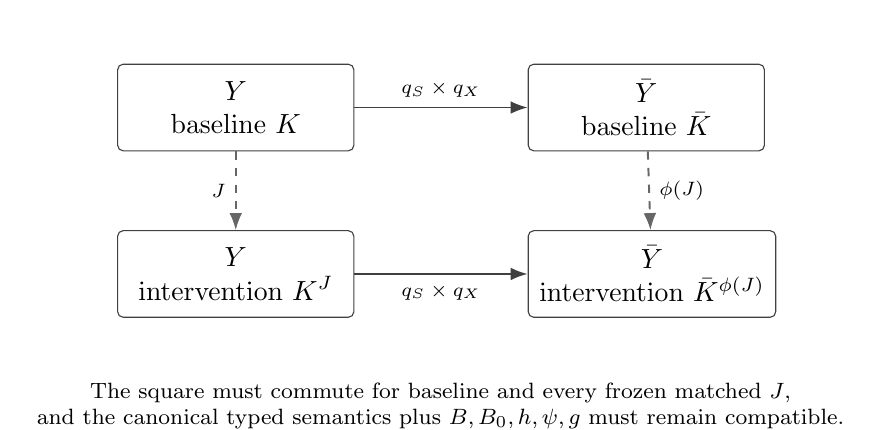
\begin{tikzpicture}[>=Latex,node distance=10mm and 22mm,
  box/.style={draw=black!75,rounded corners=2pt,fill=white,align=center,minimum width=30mm,minimum height=11mm,inner sep=4pt},
  arr/.style={->,line width=.7pt,draw=black!75},
  darr/.style={->,dashed,line width=.7pt,draw=black!60}]
\node[box] (y0) {$Y$\\baseline $K$};
\node[box, right=of y0] (yb0) {$\bar Y$\\baseline $\bar K$};
\node[box, below=of y0] (yj) {$Y$\\intervention $K^J$};
\node[box, right=of yj] (ybj) {$\bar Y$\\intervention $\bar K^{\phi(J)}$};
\draw[arr] (y0)-- node[above,font=\scriptsize] {$q_S\times q_X$} (yb0);
\draw[arr] (yj)-- node[below,font=\scriptsize] {$q_S\times q_X$} (ybj);
\draw[darr] (y0)-- node[left,font=\scriptsize] {$J$} (yj);
\draw[darr] (yb0)-- node[right,font=\scriptsize] {$\phi(J)$} (ybj);
\node[font=\footnotesize,align=center,below=7mm of yj,xshift=26mm] {The square must commute for baseline and every frozen matched $J$,\\and the canonical typed semantics plus $B,B_0,h,\psi,g$ must remain compatible.};
\end{tikzpicture}
\caption{Intervention-compatible typed quotient requirement. The state compression is type-respecting, and baseline lumpability alone is insufficient for PR preservation.}
\label{fig:quotient-diagram}
\end{figure}

\subsection{7.5 Nuisance-state padding and grounded
constitution}\label{nuisance-state-padding-and-grounded-constitution}

The stress-test motivation is an augmentation \(\ensuremath{\widetilde Y}=Y\times{}R\) in which
an auxiliary bookkeeping coordinate \(r\in{}R\) is updated by the
strategic generator but does not alter the substantive regime
observation. If a constitutive property is allowed to inspect the whole
augmented path, an intervention on the auxiliary coordinate can
manufacture \(\mathrm{PR}_{\mathrm{general}}\) status even when the
world process is unchanged. The grounded subclass prevents that result
unless the auxiliary coordinate was explicitly included in the frozen
relevance map.

Proposition 7.5 (Nuisance-padding exclusion under a fixed relevance
map). Let \(\ensuremath{\widetilde Y}=Y\times{}R\) and let \ensuremath{\widetilde g}(y,r)=g(y). Suppose a baseline model
and its intervention have the same projected g-path laws before and
after adding or modifying the auxiliary coordinate r. Then every
\ensuremath{\widetilde g}-grounded property \(\psi\) has the same baseline and post-intervention
values as in the unpadded representation. In particular, changing r
alone cannot create grounded constitutive status. If an application
intends r to be substantively regime-defining, r must be included in \ensuremath{\widetilde g}
before the counterfactual is evaluated.

Proof. By definition, a \ensuremath{\widetilde g}-grounded property factors through the
pushforward path law \((\widetilde g^\infty)_{\push}\mu\). The auxiliary
coordinate is removed by \ensuremath{\widetilde g}, and the assumed projected baseline and
post-intervention laws are unchanged. Therefore the property values and
all \(d_\psi\) gaps are unchanged. \hfill\textsc{q.e.d.}

\section{8. Canonical Examples}\label{canonical-examples}

\subsection{8.1 A periodic Generated Regime without an equilibrium
primitive}\label{a-periodic-generated-regime-without-an-equilibrium-primitive}

Let \(S=X=A=\{0,1\}\) and take every action to be feasible at every
state. Define \(\alpha(a=s\mid s,x)=1\), \(P(x'=1-a\mid s,x,a)=1\), and
\(U(s'=1-s\mid s,x,a,x')=1\). Consider the two-state subset

\begin{equation}
B=B_0=\{(0,0),(1,1)\}.
\tag{19}\label{eq:19}
\end{equation}

From (0,0), the process chooses a=0, sets \(x'=1\), and updates
\(s'=1\), reaching (1,1). From (1,1), it reaches (0,0). Thus B is
exactly invariant and the joint process has period two. Let H=Y with the
discrete topology and let \(h:Y\to{}H\) be the identity map. Then

\begin{equation}
\nu=\tfrac12\delta_{(0,0)}+\tfrac12\delta_{(1,1)}.
\tag{20}\label{eq:20}
\end{equation}

is the almost-sure limiting occupation law from either initial state.
With the counting reference measure, Assumption 4.1 is satisfied. This
is an Exact GR even though no equilibrium certificate is a primitive of
the construction. The example demonstrates that equilibrium
certification is not logically necessary to the regime-classification
layer; it does not claim that the periodic process could not also arise
from some separately specified equilibrium model, nor that periodic
dynamics are new.

\textbf{Proposition 8.1.} The tuple defined by (19)-(20) is an Exact GR
under almost-sure weak occupation convergence.

\emph{Proof.} The transition is deterministic and alternates between the
two points of B, so exact invariance is immediate. The empirical
frequency of each point differs from 1/2 by at most 1/T, giving weak
convergence of the empirical occupation measure to \(\nu\) from both
initial states. \hfill\textsc{q.e.d.}

\subsection{8.2 A discrete strategy-world feedback
loop}\label{a-discrete-strategy-world-feedback-loop}

A slightly different interpretation makes the feedback semantics
explicit. Let \(X_t\) indicate a depleted (0) or replete (1) resource
state. Let the strategic generator choose a low-impact action when the
resource is depleted and a high-impact action when it is replete. Let
the low-impact action restore the resource and the high-impact action
deplete it. The resulting deterministic loop alternates between behavior
and resource conditions. This is a discrete toy analogue of the
bidirectional strategy-environment coupling formalized in
feedback-evolving games; it is not intended as a discretization theorem
for any particular continuous-time model.

Continuous-time eco-evolutionary systems can be compared to the
canonical framework by considering a time-\(\Delta\) skeleton when the
flow or Markov process is well defined. However, exact equivalence
between continuous-time persistence and skeleton persistence requires
additional conditions: a trajectory may leave and re-enter B between
sample times. Continuous-time GRs therefore belong in a separate
extension rather than being smuggled into the discrete core.

\subsection{8.3 Same baseline regime, different
constitution}\label{same-baseline-regime-different-constitution}

Theorem 7.3 is also a substantive example. Both models generate the same
i.i.d. Bernoulli world process, the same invariant region, and the same
limiting occupation law. A baseline-only regime analysis cannot
distinguish them. Once the same action-selection intervention is
applied, one system is unaffected while the other becomes absorbed. The
difference is not an additional attractor concept; it is a statement
about which typed mechanism is constitutive of the baseline regime.

\section{9. Regime Profiles and Feedback
Diagnostics}\label{regime-profiles-and-feedback-diagnostics}

\subsection{9.1 Separate generator class from regime
class}\label{separate-generator-class-from-regime-class}

A central design rule is that generator type and regime type are
different axes. An equilibrium generator can produce a changing world
state. A learning generator can converge to a fixed point. A replicator
generator can generate a cycle. A stochastic policy can induce an
invariant distribution. The paper therefore avoids using ``equilibrium
regime'' and ``non-equilibrium regime'' as exhaustive dynamical
categories.

\begin{longtable}[]{@{}
  >{\raggedright\arraybackslash}p{(\columnwidth - 2\tabcolsep) * \real{0.5000}}
  >{\raggedright\arraybackslash}p{(\columnwidth - 2\tabcolsep) * \real{0.5000}}@{}}
\toprule\noalign{}
\begin{minipage}[b]{\linewidth}\raggedright
\textbf{Axis}
\end{minipage} & \begin{minipage}[b]{\linewidth}\raggedright
\textbf{Illustrative labels}
\end{minipage} \\
\midrule\noalign{}
\endhead
\bottomrule\noalign{}
\endlastfoot
Generator class & equilibrium-certified; best-response; fictitious-play;
reinforcement; no-regret; evolutionary; fixed policy; exogenous \\
Regime locus & world; strategic; coupled \\
Asymptotic form & fixed; periodic; recurrent; limiting-occupation;
invariant-factor (when verified); balanced-growth; contracting;
target-approaching \\
Persistence status & exact; \((L,\eta)-quasi\); QSD-certified quasi-regime; metastable extension \\
Constitution & generator-constitutive; structurally constitutive;
jointly constitutive; not established \\
Feedback & reinforcing; limiting; mixed/self-regulating; not
identified \\
\end{longtable}

Table 3. Multi-axis Generated Regime profile. Labels require explicit
mathematical or intervention-relative definitions in applications.

\subsection{9.2 Typed feedback graph}\label{typed-feedback-graph}

For interpretation, a model may carry a signed directed graph whose
nodes are components of S and X. Edges \(S\to{}X\) represent
model-implied effects of strategic variables or actions on world
dynamics; edges \(X\to{}S\) represent effects of world state on future
action selection or strategic updating. A reinforcing cycle amplifies a
predeclared regime property, a limiting cycle attenuates it, and mixed
loops can produce bounded persistence or oscillation. These graphs are
model-relative bookkeeping unless separate identification assumptions
justify a causal interpretation.

The typed graph is useful because an enlarged-state dynamical system
treats all coordinates symmetrically. The graph instead records the
analyst's structural claim about where behavior is generated and where
consequences enter. Theorem 7.2 warns that this claim cannot generally
be inferred from K alone.

\section{10. Analytical Implications}\label{analytical-implications}

\subsection{10.1 Equilibrium becomes a generator certificate, not a
regime
primitive}\label{equilibrium-becomes-a-generator-certificate-not-a-regime-primitive}

Under the generalized framework, equilibrium retains an important role
but a narrower one. It certifies a particular strategic generator or
action rule. The regime layer then asks what process that certified
behavior produces when composed with the world transition. This recovers
the original EGR logic exactly while making clear that learning,
evolutionary, or exogenous generators can feed the same regime layer
after their own behavioral assumptions are specified.

\subsection{10.2 The object is analyst-relative by
design}\label{the-object-is-analyst-relative-by-design}

A GR is not the unique ``true regime'' mechanically extracted from a
process. It is a declared classification object. This is a feature
rather than a defect, provided the declaration is ex ante and
nontrivial. Standard dynamical systems may identify maximal invariant
sets, chain-recurrent components, attractors, or ergodic measures
intrinsic to a chosen process. GR analysis instead asks whether a
specific region, descriptor, and occupation property relevant to a
substantive question is satisfied. The cost is analyst dependence; the
discipline is predeclaration, held-out validation, and explicit
convergence conditions.

\subsection{10.3 Why the typed factorization earns its
keep}\label{why-the-typed-factorization-earns-its-keep}

If the objective were only to classify the baseline trajectory, the
factorization could be discarded after forming K. Theorem 7.3 shows the
additional value: baseline dynamical equivalence does not imply
constitutive equivalence. A modeler may care not only that a regime
persists but whether it persists because agents keep selecting a
behavior, because the world mechanically amplifies that behavior,
because the learning rule reconstructs it after shocks, or because
several mechanisms are jointly necessary. These are typed counterfactual
questions.

\subsection{10.4 Implications for empirical
work}\label{implications-for-empirical-work}

The non-identification theorem imposes a hard claim boundary. Observed
state trajectories cannot by themselves generally identify \(\alpha\),
U, and P, and even full observational action support does not guarantee
that an observational conditional distribution is the causal world
mechanism preserved under an intervention. Empirical PR claims therefore
require intervention-relevant identification and an explicit account of
what is observed, estimated, structurally assumed, or externally
certified. The required evidence may come from structural restrictions,
experiments, natural experiments, valid instruments, sufficient-state
adjustment under justified assumptions, direct measurements, engineering
or institutional mechanism knowledge, or another defensible causal
design. Without that information, one may establish a GR relative to an
estimated K or path law while remaining agnostic about strategic
constitution.

This distinction mirrors the earlier EGR warning that a signed feedback
graph is not automatic causal identification and that interventions must
state what changes and what remains fixed. The generalized framework
makes the same discipline even more important because generator and
world mechanisms are separately typed. Confirmatory empirical use must
additionally audit intervention-reachable support, causal modularity,
and provenance; model-imputed off-support quantities cannot serve as the
sole evidence validating the same model that imputed them. Ambiguity is
a valid result and should be preserved rather than resolved by choosing
a convenient structural completion.

\subsection{10.5 Three-layer confirmatory
architecture}\label{three-layer-confirmatory-architecture}

The confirmatory architecture separates the formal mathematical object from the semantic
counterfactual specification and the empirical certificate. A failure in
the empirical layer downgrades the application certificate; it does not
rewrite the mathematical GR/PR object.

\begin{longtable}[]{@{}
  >{\raggedright\arraybackslash}p{(\columnwidth - 4\tabcolsep) * \real{0.3333}}
  >{\raggedright\arraybackslash}p{(\columnwidth - 4\tabcolsep) * \real{0.3333}}
  >{\raggedright\arraybackslash}p{(\columnwidth - 4\tabcolsep) * \real{0.3333}}@{}}
\toprule\noalign{}
\begin{minipage}[b]{\linewidth}\raggedright
\textbf{Layer}
\end{minipage} & \begin{minipage}[b]{\linewidth}\raggedright
\textbf{Contents}
\end{minipage} & \begin{minipage}[b]{\linewidth}\raggedright
\textbf{Failure consequence}
\end{minipage} \\
\midrule\noalign{}
\endhead
\bottomrule\noalign{}
\endlastfoot
A - Mathematical regime core & Canonical process, GR specification,
Exact GR gate, generalized PR definition, representation/intervention
theorems. & Formal GR/PR status is determined only by the mathematical
assumptions and declared intervention. \\
B - Frozen semantic counterfactual specification & State decomposition
and sufficiency; \(B,B_0,h,\nu,\mathfrak c\); relevance map g; property
\(\psi\); \(B_1\); component grammar; J; hard target closure; semantic
transport rules. & A semantic ambiguity or post-hoc switch blocks
confirmatory use unless the search is validly adjusted or held out. \\
C - Empirical certificate & Rooted provenance; intervention-reachable
support; causal identification; identified model set; outer joint
structural/statistical uncertainty; selection/multiplicity/sequential
procedure; application certificate tuple. & Failure downgrades or
invalidates the empirical certificate while leaving Layer A
unchanged. \\
\end{longtable}

Table 4. Three-layer architecture for confirmatory use. The
certification layer is an annotation on an application, not a new
mathematical regime class.

For confirmatory use, Layer B is frozen as one joint pipeline identifier
rather than as a collection of separately mutable choices. The
identifier should bind g, the component grammar, J, \(\psi/outcome\)
definition, hard structural conventions, model-set construction, and
inferential procedure. If the analyst searches across the Cartesian
product of these choices, confirmation requires a valid held-out or
selection-adjusted analysis that accounts for the search.

The provenance record in Layer C should be an acyclic rooted derivation
graph rather than a flat list. Every empirical assumption must
ultimately trace to admissible external evidence, a formally declared
identity/axiom, or an independently certified upstream result. Circular
support does not become valid merely because every node has a citation
to another node in the same cycle.

\subsection{10.6 Partial identification and outer uncertainty
sets}\label{partial-identification-and-outer-uncertainty-sets}

When evidence identifies a provenance-valid set of structural models M
rather than one model, confirmatory PR classification must quantify over
the full set rather than a representative, average, majority,
posterior-majority, or convenient witness. For a declared protocol,
robust pointwise PR requires a nonzero constitutive effect for every
\(m\in{}M\) and every \(y\in{}B_1\). Robust uniform PR additionally
requires one common positive \(d_\psi\) gap over the same joint set.

Applications should separate three questions: (i) PR status - whether
constitution is nonzero throughout the admissible model/state set; (ii)
direction - whether the sign is common; and (iii) uniform gap - whether
one \(\delta_\psi>0\) works over the entire admissible set. Robust PR
can therefore coexist with direction ambiguity, and pointwise robustness
need not imply a common positive uniform gap.

If the identified set is estimated from finite data, structural and
sampling uncertainty must be combined into one valid outer joint
model/effect set before classification. Intersecting per-model
confidence sets, averaging effects, or classifying uncertainty layers
separately can manufacture certainty. When a valid covered outer set
still contains a zero-constitution case, the statistical status is
\texttt{STATISTICALLY\_UNRESOLVED}. Failure to statistically certify PR
is not, by itself, evidence of nonconstitution.

The statistical procedure must have justified coverage for the actual
inferential object. Where relevant this includes simultaneous coverage
over \(B_1\), multiple interventions, model-set endpoints,
data-dependent selection, and sequential monitoring. Fixed-sample
marginal intervals are not automatically valid after optional stopping
or post-hoc intervention search; multiplicity correction cannot repair
an intrinsically under-covering base procedure.

\subsection{10.7 Orthogonal application
certificate}\label{orthogonal-application-certificate}

The application-status vocabulary is not a mutually exclusive
enumeration. A confirmatory report should retain an orthogonal
certificate tuple so one dimension cannot erase another. A compact
headline may be derived for presentation, but the underlying tuple
should remain auditable.

\begin{table}[htbp]
\centering
\footnotesize
\caption{Orthogonal application-certificate tuple. These are reporting annotations, not additional GR/PR theorem classes.}
\label{tab:certificate}
\begin{tabularx}{\textwidth}{@{}>{\raggedright\arraybackslash}p{.26\textwidth}X@{}}
\toprule
\textbf{Dimension} & \textbf{Illustrative values}\\
\midrule
Validity & \status{VALID}; \status{INVALID}\\
Epistemic mode & \status{FORMAL_THEORETICAL}; \status{EMPIRICAL_CONFIRMATORY}; \status{EMPIRICAL_EXPLORATORY}; \status{ASSUMPTION_CONDITIONAL}\\
Selection status & \status{FROZEN_REGISTERED}; \status{HELD_OUT_OR_SELECTION_ADJUSTED}; \status{POST_HOC_EXPLORATORY}\\
Identification status & \status{POINT_IDENTIFIED}; \status{SET_IDENTIFIED}; \status{STRUCTURALLY_UNRESOLVED}\\
Statistical status & \status{NOT_APPLICABLE}; \status{RESOLVED_AT_DECLARED_COVERAGE}; \status{STATISTICALLY_UNRESOLVED}\\
Provenance status & \status{SUPPORTED}; \status{INSUFFICIENT}; \status{NOT_APPLICABLE}\\
Substantive PR status & \status{ROBUST_PR}; \status{ROBUST_NONCONSTITUTIVE_UNDER_FROZEN_PROTOCOL}; \status{PR_STATUS_AMBIGUOUS}; \status{NOT_EVALUATED}\\
Direction status & \status{POSITIVE}; \status{NEGATIVE}; \status{DIRECTION_AMBIGUOUS}; \status{NOT_APPLICABLE}\\
Uniform-gap status & \status{ESTABLISHED}; \status{UNRESOLVED}; \status{NOT_APPLICABLE}\\
\bottomrule
\end{tabularx}
\end{table}

\section{11. Extensions Beyond the Canonical Discrete-Time
Core}\label{extensions-beyond-the-canonical-discrete-time-core}

\subsection{11.1 Continuous time}\label{continuous-time}

A continuous-time version replaces the discrete joint kernel by a flow,
semigroup, stochastic differential equation, or controlled generator on
\(S\times{}X\), while retaining a typed decomposition of strategic and
world dynamics. For deterministic models one natural form is

\begin{equation}
\dot S_t=F_S(S_t,X_t),\qquad \dot X_t=F_X(S_t,X_t).
\tag{21}\label{eq:21}
\end{equation}

with \(F_S\) interpreted as strategic-generation/update dynamics and
\(F_X\) as world dynamics. Eco-evolutionary games fit this template
directly. The corresponding GR definition would use forward invariance,
occupation measures, recurrent sets, or other continuous-time asymptotic
descriptors. Because continuous trajectories can exit a region between
discrete sample times, continuous-time exact persistence should be
defined directly rather than inferred from a time-skeleton.

\subsection{11.2 Differential inclusions and set-valued
generators}\label{differential-inclusions-and-set-valued-generators}

Best-response correspondences, discontinuous adaptation, and some
bounded-rational processes are more naturally represented by
differential inclusions or set-valued dynamics. Benaïm, Hofbauer, and
Sorin (2005) already supply an appropriate asymptotic substrate through
internally chain-transitive sets and attractors. A continuous-time PR
extension should reuse that mathematics and add only the typed regime
and intervention semantics.

\subsection{11.3 Nonautonomous and random
generators}\label{nonautonomous-and-random-generators}

If the generator or world law changes exogenously with time, the
appropriate baseline object may be a nonautonomous process or cocycle
rather than a stationary Markov kernel. Kloeden and Rasmussen (2011)
develop process and skew-product formulations, pullback attractors,
switching systems, and random dynamical systems. A future nonautonomous
PR should therefore index the strategic generator and world law by time
or an external driving process, for example \(\mathfrak G_t\) and
\(P_t\), and replace stationary occupation assumptions where necessary.
This extension lies outside the discrete-time framework developed here.

\subsection{11.4 Partial observability and belief
states}\label{partial-observability-and-belief-states}

Partially observed strategic systems can often be made Markov by
augmenting S with sufficient beliefs, filters, or internal information
states. When no finite- or countable-dimensional sufficient statistic
exists, the strategic state may itself be a probability measure or other
infinite-dimensional object. The Polish-space core accommodates many
such cases, but application-specific existence and measurability
conditions must be checked.



\section{12. Falsifiability, Failure Modes, and Claim
Boundary}\label{falsifiability-failure-modes-and-claim-boundary}

\subsection{12.1 Ways the framework can
fail}\label{ways-the-framework-can-fail}

The framework is intentionally falsifiable at several levels.

\begin{itemize}
\item
  Well-posedness failure: \(\alpha\), U, or P is not measurable or does
  not preserve feasibility, so the canonical process is undefined.
\item
  Regime-specification failure: B, \(B_0\), h, \(\nu\), or the
  convergence mode is chosen after observing the evaluated trajectory or
  is trivial under Assumption 4.1.
\item
  Persistence failure: the declared B is not exactly invariant, so the
  object is not an Exact GR.
\item
  Occupation failure: the empirical descriptor measures do not converge
  to the declared \(\nu\) under the stated mode for all admissible
  initial laws.
\item
  Protocol-relative constitution failure: under the frozen intervention
  protocol, the proposed strategic component can be intervened upon
  without changing \(\psi\) on the declared comparison set. This
  excludes constitution under that protocol; it does not by itself
  exclude every other admissible intervention family.
\item
  Identification failure: available evidence establishes only K or a
  path law, or leaves intervention-relevant mechanism rows/model
  completions unresolved, so the decomposition/counterfactual required
  for a strategic constitutive claim is not identified.
\item
  Numerical pseudo-exactness: floating-point equality or a tolerance is
  used to promote a leaky process to Exact GR; exact claims require
  analytic, symbolic/rational, certified-interval, proof-object, or
  equivalent exactness support.
\item
  Statistical-certification failure: the confidence region undercovers
  the actual joint inferential object, ignores multiplicity or optional
  stopping, or a zero-containing valid set is treated as resolved PR
  status.
\item
  Partial-identification overreach: admissible models disagree about
  constitution but the application reports a representative, average,
  majority, or single-witness classification as if status were
  identified.
\item
  Provenance failure: an empirical assumption is supported only by a
  circular/rootless derivation graph, post-hoc hard/soft labeling, or a
  model-imputed quantity that is used to validate the same model.
\item
  Intervention-support/modularity failure: the intervention reaches
  unsupported rows or relies on held-fixed causal mechanisms whose
  stability under J lacks adequate identification/provenance.
\item
  Empirical-admissibility failure: a formally typed intervention
  violates a predeclared hard structural relation outside its declared
  target, or the target is not closed under the hard dependency
  relation.
\item
  Relevance/semantic-selection failure: g, the component grammar,
  \(\psi\), J, or another semantic counterfactual element is chosen
  after seeing the result without a valid held-out or selection-adjusted
  procedure.
\item
  State-sufficiency failure: the observed or aggregated state is treated
  as Markov without a valid lumpability/sufficiency argument; hidden
  states within one aggregate label can therefore induce different
  continuation laws.
\item
  Reduction failure of novelty: if a proposed application uses only
  baseline attractors or invariant sets and no typed intervention
  semantics, standard dynamical-systems language may be sufficient and
  PR terminology may add nothing.

\item
  QSD overclaim: a QSD is invoked without proving existence for the killed kernel, or uniqueness is assumed where several QSDs can coexist.
\item
  Perturbation overreach: a finite-horizon perturbation bound is extrapolated to stationary or infinite-path behavior without the ergodic, contraction, spectral, or killed-process assumptions needed for such a step.
\item
  Margin-boundary failure: a robustness claim uses \(\kappa\ge\varepsilon_0+\varepsilon_J\) rather than the strict certificate \(\kappa>\varepsilon_0+\varepsilon_J\), or treats pointwise nonzero effects as a positive uniform margin.
\item
  Intervention-family omission: an equivalence claim matches only a subset of frozen intervention kernels, or chooses the family after observing which counterfactuals agree.
\item
  Quotient overreach: a state quotient is only baseline-lumpable while an intervention kernel, regime set, descriptor, property map, relevance map, or admissible initial-law class fails to descend.
\item
  Rigidity-domain failure: a candidate scalar-defect, finite-detection, first-bad, singular-compatibility, or witness theorem is applied outside the subclass that supplies its hypotheses.
\end{itemize}

\subsection{12.2 Nonclaims}\label{nonclaims}

The canonical formulation does not establish equilibrium existence for
arbitrary games; universal convergence of learning; empirical causal
identification from observational trajectories; general recurrence or
ergodicity of K; existence of limiting occupation laws for arbitrary
generators; equivalence between metastability and exact persistence; or
a complete continuous-time, nonautonomous, or
differential-inclusion PR theory. These must be supplied by the
underlying model or the neighboring mathematical literature. It also
does not imply that a relevance map, component decomposition, causal
factorization, identified model set, or inferential procedure is
uniquely recoverable from baseline trajectories; nor does an application
certificate supplied by Section 10 convert assumption-dependent evidence
into point identification.

\subsection{12.3 Novelty standard}\label{novelty-standard}
The relevant novelty test is functional rather than terminological. Mature adjacent literatures already contain most mathematical ingredients used here. Labelled Markov-process theory supplies bisimulation and behavioral metrics for label-indexed kernel families; causal-abstraction theory studies preservation of interventional predictions across representations; killed-process theory supplies QSD and exit-time machinery; and Markov perturbation theory supplies kernel-to-law sensitivity bounds under explicit regularity assumptions. Accordingly, this paper does not claim novelty for those ingredients, nor for the broad observation that baseline equivalence can coexist with intervention nonequivalence. The framework-specific claim is narrower: a typed strategic/world regime layer that combines ex ante GR semantics, predeclared constitutive generator interventions, grounded confirmatory semantics, exact persistence calculus, quantitative margin certification, and sufficient family-compatible quotient conditions in one portable object. That assessment remains provisional and should be revised if a prior framework is shown to provide the same combined function.

\section{13. Conclusion}\label{conclusion}

The original EGR question was asked after equilibrium: once a strategic
policy is certified, what persistent world does it generate? The
generalized formulation shows that equilibrium is not a primitive of the
regime layer. It is one possible certificate for a strategic generator.
A learning rule, evolutionary protocol, fixed policy, or other
sufficiently specified behavioral process can generate the same kind of
regime-classification problem.

At the same time, the framework does not replace dynamical-systems or Markov-process mathematics. The joint process is an ordinary Markov process on an enlarged state, and its invariant sets, recurrence, occupation measures, killed-process behavior, or metastability should be analyzed with established tools. The additional object is typed and intervention-relative. A Generated Regime classifies a declared persistent process. A Permansson Regime adds the claim that a specific component of the strategic generator is constitutive of a defining regime property under an admissible intervention.

The quantitative layer makes this separation sharper. Polish descriptor spaces broaden the ambient class; killed kernels provide exact finite-persistence and exit-time identities; QSDs furnish an optional finite-horizon certificate; constitutive margins quantify robustness to bounded property-output error; frozen intervention-family signatures extend representation equivalence; and the quotient theorem gives sufficient conditions under which GR/PR semantics survive type-respecting state compression. These results do not replace the application disciplines of relevance, component grammar, causal modularity, support, provenance, identification, or statistical uncertainty.

The central result is therefore the separation between baseline dynamical equivalence and constitutive equivalence. Two models may generate the same baseline joint process and the same long-run regime while responding differently to strategic intervention. Conversely, when baseline and matched intervention kernels and the relevant semantics agree, the corresponding constitutive classifications agree. The Permansson layer preserves the typed intervention information needed to ask not only what regime a process generates, but which strategic mechanisms are constitutive of that regime.

\section{14. Appendix A - Compact Theorem and Definition Ledger}\label{appendix-a---compact-theorem-and-definition-ledger}

\begin{table}[htbp]
\centering
\footnotesize
\caption{Core GR/PR theorem and definition ledger.}
\label{tab:core-ledger}
\begin{tabularx}{\textwidth}{@{}>{\raggedright\arraybackslash}p{.30\textwidth}X@{}}
\toprule
\textbf{Item} & \textbf{Core statement}\\
\midrule
Joint-process construction & $\alpha$, $P$, and $U$ compose into $K_{\mathfrak G,P}$; Ionescu--Tulcea gives a unique path law.\\
Exact GR & Ex ante specification + exact invariance of $B$ + limiting descriptor occupation law for all $\lambda$ supported on $B_0$.\\
Generalized PR & Exact GR + at least one strategic-generator component constitutive under a fixed admissible $J^{\mathfrak G}$.\\
EGR embedding & Use $S_E=\mathbb N_0\times(A\cup\{\bot\})$ to record clock and previous action; $\alpha=\delta_{\pi^\ast}$, $U$ records the realized action, and the $X$-marginal equals the Paper-I equilibrium-induced kernel.\\
Conservative PR extension & Paper-I date/state policy interventions map to clock-indexed action-selection interventions; under a well-defined frozen Paper-I descriptor/property convention, baseline and counterfactual executions and constitutive comparisons are preserved.\\
Baseline representation invariance & Same $K$ + same $\Sigma$ + same reference-measure convention $\Rightarrow$ same GR classification.\\
Factorization non-identification & Same $K$ does not imply same $\mathfrak G$ or $P$.\\
Constitutive non-invariance & Same baseline $K$ can yield different PR status under the same typed intervention.\\
Intervention-compatible invariance & If both baseline and matched post-intervention $K$ coincide, constitution classification coincides.\\
\bottomrule
\end{tabularx}
\end{table}

\begin{table}[htbp]
\centering
\footnotesize
\caption{Quantitative and representation-theoretic results.}
\label{tab:quant-ledger}
\begin{tabularx}{\textwidth}{@{}>{\raggedright\arraybackslash}p{.30\textwidth}X@{}}
\toprule
\textbf{Item} & \textbf{Core statement}\\
\midrule
Polish descriptor-space generality & $H$ may be any Polish descriptor space equipped with a bounded compatible metric; $d_{\mathrm{BL}}$ still metrizes weak convergence. No existence/tightness conclusion is automatic.\\
Exact killed-kernel persistence & For $y\in B$, $P_y(\tau_B>n)=K_B^n\mathbf1_B(y)$, and $E_y[\tau_B]=\sum_{n\ge0}K_B^n\mathbf1_B(y)$ as an extended identity.\\
QSD-certified quasi-regime & An $(L,\eta)$-quasi-regime may carry an additional QSD certificate $\mu_BK_B=\theta_B\mu_B$; then survival from $\mu_B$ is $\theta_B^n$ and the conditional law given survival is $\mu_B$. The QSD equation does not replace the uniform finite-persistence gate, and existence/uniqueness require separate hypotheses.\\
Constitutive robustness margin & Uniform property-output errors $\varepsilon_0,\varepsilon_J$ imply $|\widetilde\kappa-\kappa|\le\varepsilon_0+\varepsilon_J$; $\kappa>\varepsilon_0+\varepsilon_J$ certifies persistence of uniform constitution.\\
Intervention-family invariance & A frozen target/type-grammar-preserving matching of the indexed intervention family, with equal baseline and matched $K^J$, implies identical corresponding effect profiles, uniform margins, and protocol-scoped classifications.\\
Intervention-compatible quotient preservation & Between two canonical typed models under a type-respecting product map q, if the baseline and every frozen matched intervention kernel intertwine, both comparison sets remain admissible, and $B,B_0,h,\psi,g$ plus initial-law lifting are compatible, GR/PR classification descends and lifts.\\
\bottomrule
\end{tabularx}
\end{table}

The relevance, intervention, provenance, identified-set, and statistical rules are application/certification disciplines surrounding the mathematical core. The persistence, robustness, family-equivalence, and quotient results above do not alter the set-theoretic hierarchy of GR, $\mathrm{PR}_{\mathrm{general}}$, $\mathrm{PR}_g$, or the transported Paper-I subclass. The specialized finite-certificate and rigidity material in Appendix E lies outside this core ledger.

\section{15. Appendix B - Proof Notes and Technical
Clarifications}\label{appendix-b---proof-notes-and-technical-clarifications}

\subsection{15.1 Measurability of the composed
kernel}\label{measurability-of-the-composed-kernel}

For bounded measurable \(f:Y\to{}\mathbb R\), define the Markov operator

\begin{equation}
(Kf)(s,x)=\int_A\!\int_X\!\int_S f(s',x')\,U(ds'\mid s,x,a,x')\,P(dx'\mid s,x,a)\,\alpha(da\mid s,x).
\tag{22}\label{eq:22}
\end{equation}

Successive kernel integration preserves measurability. Taking
\(f=\mathbf 1_E\) yields (6). This is the standard kernel-composition
argument used in controlled Markov processes and does not require a new
existence theorem.

\subsection{15.2 Why the descriptor is
global}\label{why-the-descriptor-is-global}

The earlier EGR definition used \(h:B\to{}H\) because exact equilibrium
persistence keeps the baseline path inside B. In the generalized
intervention setting, the counterfactual process may leave B precisely
because the intervention destroys a defining regime property. Defining h
globally avoids an unnecessary extension step. For the EGR embedding,
any constant Borel extension outside B preserves all baseline EGR
claims. For the conservative Permansson theorem, however, if a Paper-I
property functional evaluates h after an intervention exits B, the
extension must be part of the frozen intervention/descriptor convention;
the theorem does not manufacture an ex post value for an otherwise
undefined Paper-I descriptor.

\subsection{\texorpdfstring{15.3 Why \(B_1\) has at least two initial
states}{15.3 Why B\_1 has at least two initial states}}\label{why-b_1-has-at-least-two-initial-states}

A constitutive claim evaluated at a single hand-picked initial condition
can be fragile and can collapse into a trajectory-specific sensitivity
statement. The Paper-I wording therefore requires at least two initial
states. Because full point-initialized path laws include their
deterministic time-zero coordinate, ``distinct path laws'' is no
stronger than ``distinct states'' unless a continuation-law qualifier is
added. Distinct shifted continuation laws remain a useful diagnostic,
but the framework does not treat them as a universally strongest guardrail. For
grounded confirmatory work, an optional stronger audit can compare
g-projected baseline/intervention response profiles: two states are
substantively distinguishable when their grounded path laws differ at
baseline or under the frozen counterfactual. Even this is a diagnostic
rather than a universal gate, because latent types, beliefs, and
learning states can pool under baseline observations yet respond
differently under J. None of these diversity diagnostics substitutes for
a defensible predeclared relevance map. Uniform constitution strengthens
the substantive comparison by imposing a positive \(d_\psi\) separation
over \(B_1\). Basin-only or pooled-baseline classifications should be
described transparently rather than rejected by a rule that would also
exclude legitimate contraction and hidden-state models.

\subsection{15.4 Why exact GR requires invariance on all of
B}\label{why-exact-gr-requires-invariance-on-all-of-b}

If exact persistence were required only from \(B_0\), the analyst could
place unreachable leakage states inside B and still label B a regime
region. Requiring \(K(B\mid y)=1\) for every \(y\in{}B\) makes B
genuinely invariant. The initial basin \(B_0\) then controls which
subset of the invariant region is claimed to share the declared
occupation law.

\subsection{15.5 Why equality of baseline K is not enough for PR
equivalence}\label{why-equality-of-baseline-k-is-not-enough-for-pr-equivalence}

A factorization defines a counterfactual grammar. Theorem 7.2 shows that
many grammars can induce the same baseline K. Permansson constitution is
therefore not a function of K alone; it is a function of the baseline
process plus the typed intervention map. Proposition 7.4 states the
appropriate invariance condition for matched interventions. Proposition
7.5 adds the representation guard: a confirmatory property is evaluated
only through a frozen relevance map g, so nuisance coordinates omitted
from g cannot manufacture grounded PR status. This does not make
substantive relevance mathematically automatic; it forces the analyst to
declare which coordinates are allowed to matter before the
counterfactual is seen.

\subsection{15.6 Why empirical admissibility is separate from typed
intervention}\label{why-empirical-admissibility-is-separate-from-typed-intervention}

A typed intervention is a mathematical surgery on declared kernels. That
is sufficient to define the formal counterfactual but not to establish
that the same surgery is empirically meaningful in a real system. Hard
structural identities can force the effective target to expand;
intervention-reachable rows may lie outside baseline support; and an
observational conditional distribution may differ from the causal
mechanism that remains fixed under intervention. These are evidence and
model-identification questions, so they are treated as
certificate-layer requirements rather than alterations to Definition 5.1.

\subsection{15.7 Why negative claims are
protocol-scoped}\label{why-negative-claims-are-protocol-scoped}

Permansson constitution is defined relative to a property map,
intervention protocol, and comparison set. A null result for one J
therefore establishes only nonconstitution under that frozen protocol. A
global absence claim requires exhaustion of a predeclared admissible
intervention family or an independent theorem excluding the family. This
scope rule prevents failure of one intervention from being interpreted as
the much stronger statement that no strategically constitutive
intervention exists.

\subsection{15.8 Why uncertainty is classified through one outer
set}\label{why-uncertainty-is-classified-through-one-outer-set}

Structural ambiguity and sampling uncertainty can interact. The safe
object for confirmatory classification is therefore one outer joint set
containing every model/effect configuration retained by the
provenance-valid structural restrictions and the declared statistical
coverage procedure. Intersecting separately valid per-model confidence
sets, averaging model effects, or classifying structural and sampling
uncertainty in separate passes can remove zero-effect possibilities
without justification. Robust PR, direction, and uniform-gap claims are
assigned only after this outer set has been constructed.


\subsection{15.9 Polish descriptors and bounded-Lipschitz convergence}\label{polish-descriptors-proof-note}

Compactness was stronger than the core definition required. A Polish space admits a complete separable compatible metric $\rho$; truncating it to $\min\{1,\rho\}$ preserves the topology and completeness while making it bounded. The associated bounded-Lipschitz/Fortet--Mourier metric metrizes weak convergence of probability measures. This justifies the replacement in Section 4.1. It does not supply uniform tightness for an arbitrary family of measures, so the existence of $\nu$ remains part of Exact-GR certification rather than a topological consequence (Dudley, 2002).

\subsection{15.10 Exact killed-kernel indexing}\label{killed-kernel-indexing-proof-note}

The convention $\tau_B=\inf\{t\ge0:Y_t\notin B\}$ means that, from $y\in B$, survival beyond n is exactly retention at times 1 through n. This is why $K_B^n$ rather than $K_B^{n+1}$ appears in (11b). The $n=0$ identity is one, the induction step integrates only over B, and the Green-series formula follows from the tail-sum identity. This convention is fixed throughout the paper to prevent off-by-one ambiguity.

\subsection{15.11 QSD claims are conditional}\label{qsd-conditional-proof-note}

Equation (13a) is an eigenmeasure relation for the sub-Markov kernel. It implies geometric survival and conditional stationarity algebraically, but it neither proves that such a probability measure exists nor that it is unique. Those are separate killed-process theorems. The paper therefore uses QSD only as an additional certificate for an already established finite-horizon quasi-regime and never treats QSD, Yaglom limit, and quasi-ergodic law as synonyms. The eigenmeasure equation alone does not establish the uniform finite-persistence gate in (11).

\subsection{15.12 Why the perturbation theorem is only a bridge}\label{perturbation-bridge-proof-note}

Proposition 5.2 is pure metric geometry: it begins after errors in property-output space have already been bounded. Obtaining those errors from a kernel perturbation requires additional assumptions. Proposition 5.4 supplies a finite-horizon bound with no ergodicity requirement; long-run bounds must instead be imported from the appropriate uniform-ergodic, contraction, spectral, or killed-process theory. This modularity prevents a local one-step perturbation statement from being overextended to infinite-horizon behavior.

\subsection{15.13 Why a full intervention signature is required}\label{full-signature-proof-note}

A family claim is a conjunction over the frozen intervention labels. Equality of the baseline and one post-intervention kernel proves equivalence only for that matched label. If an omitted label produces different $K^J$, its effect profile can differ even though all checked labels agree. Proposition 7.4a therefore requires the entire predeclared indexed signature relevant to the claim and a target/type-grammar-preserving label matching; selecting either the family or its matching after inspection is outside the representation theorem.

\subsection{15.14 Why quotient preservation needs more than lumpability}\label{quotient-proof-note}

Ordinary lumpability concerns one kernel. A PR claim concerns a baseline path law, one or more intervention path laws, and frozen semantics. Theorem 7.4b therefore starts with two well-posed canonical typed models and a type-respecting product state map, requires a target/type-grammar-preserving intervention matching, kernel intertwining for every frozen label, a common property metric, and factorization of $B,B_0,h,\psi$ and, when applicable, g. The comparison sets must independently satisfy the Section 5.4 admissibility guard. The initial-law lifting assumption is included because Exact GR quantifies over every admissible initial law in the quotient basin; pointwise kernel intertwining alone does not automatically provide a measurable lift for every quotient law. Non-triviality is checked separately on each specification because interior, reference-measure positivity, descriptor diversity, and comparison-set admissibility are not invariant under arbitrary quotients.

\section{16. Appendix C - Suggested Empirical and Computational
Workflow}\label{appendix-c---suggested-empirical-and-computational-workflow}

For applied work, the following sequence keeps the claim boundary
auditable:

1. Declare the typed state decomposition \(S\times{}X\). Establish
Markov sufficiency/lumpability for any observed or aggregated state,
augment the state when necessary, or fail closed on Exact-GR
certification.

2. Specify \(\alpha\), P, and U or an estimable/identified
approximation, and distinguish observed quantities, estimated
quantities, formal identities, and structural assumptions.

3. Freeze B, \(B_0\), h, \(\nu\), \(\mathfrak c\), and any
reference-measure convention before confirmatory evaluation.

4. Verify exact invariance with an exact mathematical argument. For finite-horizon analysis, construct $K_B$ and compute or bound $K_B^L\mathbf1_B$ rather than relying only on a one-step $q^L$ diagnostic. If a QSD certificate is claimed, establish the eigenmeasure relation and any existence, uniqueness, Yaglom-limit, or quasi-ergodic claims separately; a QSD equation does not replace the finite-persistence gate. Do not promote tolerance-based or raw floating-point equality to Exact GR; otherwise report finite-horizon/quasi/metastable evidence.

5. Establish descriptor occupation convergence under the declared mode.
Verify basin-reachable descriptor nondegeneracy for confirmatory
certification and report separately whether forward descriptor richness
is satisfied.

6. Define and audit the relevance map g. Verify factorization of B and h
and grounding of \(\psi\); search strict coarsenings when feasible;
report non-unique sufficient maps; and rerun defensible alternatives
when semantics are not unique.

7. Freeze one joint semantic pipeline identifier containing g, \(\psi\),
\(B_1\), the component grammar, J, hard structural target/transport
conventions, model-set construction, and the inferential procedure. If
selection occurs, use held-out or valid selection-adjusted confirmation.

8. Conduct a component/intervention audit. Record whether the target is
atomic, compound, or joint; test substantively meaningful granularity
changes; transport interventions semantically under reparameterization;
and avoid claiming a uniquely intrinsic constitutive component without
evidence.

9. Compute hard structural target closure. If preserving a hard identity
requires additional components to move, expand/retype the target or
declare the proposed intervention inadmissible under that structural
specification.

10. Audit intervention-reachable support and causal modularity. Identify
every mechanism row that becomes relevant under J and state the evidence
supporting stability of held-fixed mechanisms.

11. Build an acyclic rooted provenance graph for hard constraints,
relevance choices, causal assumptions, support claims, model
restrictions, and upstream certificates. Reject circular or
self-validating support.

12. Construct the full provenance-valid identified model set M. Do not
substitute one representative, average, majority, posterior-majority, or
convenient model when the evidence leaves several models admissible.

13. Evaluate baseline and intervened path laws under the same frozen descriptor, relevance map, property map, and protocol for every required $m\in M$ and $y\in B_1$. Compute $\Delta_{\psi,J}(y)$ and, when uniform status is claimed, $\kappa_{\psi,J}(B_1)$. If the analysis uses approximated or estimated property outputs, propagate a justified two-sided error envelope and report whether $\kappa$ exceeds the full baseline-plus-intervention error budget.

14. Assign protocol-scoped substantive status. Report robust PR, sign/direction, and uniform-gap status separately; report \status{ROBUST_NONCONSTITUTIVE_UNDER_FROZEN_PROTOCOL} for a negative result under one J; reserve a family-wide absence or equivalence claim for an exhausted predeclared intervention family or theorem. For family comparisons, freeze and audit the full intervention signature rather than a favorable subset of labels.

15. When quantities are estimated, build one outer joint
structural/statistical uncertainty set with justified simultaneous
coverage for every dimension used by the claim. Account for multiple
interventions, model selection, data-dependent search, and sequential
monitoring/optional stopping as applicable.

16. If the valid outer set still contains a zero-constitution case,
report \texttt{STATISTICALLY\_UNRESOLVED} rather than PR or not-PR.
Non-significance does not establish nonconstitution.

17. Emit the orthogonal application-certificate tuple: validity,
epistemic mode, selection status, identification status, statistical
status, provenance status, substantive protocol-scoped outcome, and
uniform-gap status.

18. Preserve exploratory work as exploratory. Candidate regimes,
relevance maps, model restrictions, or interventions discovered on
development data require held-out or otherwise independent validation
before being treated as confirmatory empirical results.

\section{17. Appendix D - Formal Verification and Reproducibility}\label{appendix-d-formal-verification}

\subsection{17.1 Verification architecture}\label{verification-architecture}

The verification record has two deliberately separate layers. The first is executable and destructive: a frozen regression archive exercises historical controls, mutation cases, finite counterexamples, boundaries, pathologies, and representation failures. Its role is to expose mismatches between the manuscript contract and executable finite constructions. Passing those tests does not prove a universal theorem.

The second layer is deductive. The companion repository \url{https://github.com/HMarcusWH/PermanssonLean} formalizes the discrete mathematical core in Lean 4 against pinned mathlib dependencies. Its CI root build performs an axiom audit, runs \texttt{lake build}, and rejects \texttt{sorry}, \texttt{admit}, and source-level custom \texttt{axiom} declarations in the project source tree. The Lean development therefore checks the encoded theorem statements and their dependency chain against Lean's trusted kernel. This is a statement about the formalized mathematics, not about empirical truth, identification, provenance quality, or novelty.

\subsection{17.2 Machine-checked scope}\label{machine-checked-scope}

The discrete GR/PR mathematical core through Proposition 8.1 has corresponding Lean closure. The machine-checked scope includes joint-process construction and uniqueness; enlarged-state reduction; Polish descriptor-space support; exact and killed-kernel persistence; QSD-certified quasi-regimes; generalized and uniform Permansson constitution; perturbation robustness; the finite-horizon TV envelope; baseline, intervention-family, and quotient preservation; Paper-I world-only, recorded-action, and grounded transport; the Section 7 non-identification and nuisance-padding results; and the explicit period-two Exact GR witness.

This formalization scope is intentionally narrower than the full manuscript. The specialized finite-certificate and rigidity material in Appendix E is not part of the formalized universal theorem set. Continuous-time, differential-inclusion, nonautonomous, and application-specific extensions also remain outside the discrete-core claim. The application disciplines concerning relevance, causal modularity, support, provenance, identification, and statistical uncertainty also remain separate from the pure formal derivations.

\subsection{17.3 Paper-to-Lean crosswalk}\label{paper-lean-crosswalk}

\begin{table}[htbp]
\centering
\scriptsize
\caption{Primary paper-to-Lean verification crosswalk. The repository's \texttt{docs/FORMALIZATION\_MAP.md} gives the complete dependency ledger.}
\label{tab:paper-lean-crosswalk}
\begin{tabularx}{\textwidth}{@{}p{0.15\textwidth}p{0.32\textwidth}X@{}}
\toprule
Paper item & Mathematical object & Primary Lean closure \\
\midrule
Thm. 3.1 & Joint-process well-posedness & \nolinkurl{joint_process_well_posed} \\
Prop. 3.2 & Enlarged-state reduction & \nolinkurl{enlarged_state_reduction} \\
Prop. 4.1a & Polish descriptor-space generality & \nolinkurl{proposition_4_1a} \\
Prop. 4.2 / Thm. 4.2a & Exact invariance and killed persistence & \nolinkurl{exactInvariant_iff_survivalForever}; \nolinkurl{survivalProbability_eq_killedSurvivalMass} \\
Def. 4.4a / Prop. 4.4b & QSD-certified quasi-regime & \nolinkurl{IsQSDCertifiedQuasiRegime}; \nolinkurl{proposition_4_4b} \\
Prop. 5.2 / Cor. 5.3 & Constitutive-margin robustness & \nolinkurl{constitutiveMargin_perturbation_abs_le}; \nolinkurl{robustUniformPRCertificate} \\
Prop. 5.4 & Finite-horizon kernel-to-path TV envelope & \nolinkurl{proposition_5_4} \\
Thm. 6.1 & EGR embedding & \nolinkurl{paperIEGR_iff_embeddedExactGR} \\
Thm. 6.2 & Conservative Paper-I recovery & \nolinkurl{paperIPermansson_iff_embeddedRelativePR} plus recorded-action and grounded analogues \\
Prop. 7.1--7.4a & Representation and intervention-family invariance & \nolinkurl{exactGR_iff_of_inducedKernel_eq}; \nolinkurl{frozenFamilyPR_iff_of_signature_match} \\
Thm. 7.4b / Prop. 7.5 & Quotient preservation and nuisance-padding exclusion & \nolinkurl{quotient_frozenFamilyPR_iff}; \nolinkurl{nuisancePadding_cannot_create_grounded_change} \\
Prop. 8.1 & Periodic Exact GR & \nolinkurl{PeriodicExactGR.proposition_8_1} \\
\bottomrule
\end{tabularx}
\end{table}

\subsection{17.4 Reproducibility record}\label{formal-reproducibility-record}

The formalization is pinned to Lean 4.34.0 and mathlib v4.34.0. The immutable formalization snapshot used for this manuscript is commit \nolinkurl{\LeanSnapshotCommit}, whose root Lean workflow completed successfully in CI run \texttt{\LeanCIRun}. The accompanying verification manifest records SHA-256 hashes for the final PDF, the final \texttt{.tex} source, and the frozen v0.1.7 post-proofread test archive. This creates a bidirectional provenance chain: the paper identifies the exact formalization commit, and the repository-side manifest identifies the exact paper and destructive-test artifacts associated with the release.

\subsection{17.5 Revision and artifact lineage}\label{revision-artifact-lineage}

The release history is retained here for reproducibility rather than as part of the theory exposition. The v0.1.6 manuscript serves as the earlier control lineage for the generalized framework and its initial formalization record. The v0.1.7 line adds the quantitative and representation-theoretic theorem layer and the associated destructive differential suite (Runs 17--30), covering killed-kernel indexing, QSD pathologies, noncompact descriptors, finite- versus infinite-horizon perturbations, constitutive-margin boundaries, intervention-family omissions, quotient failures, and the specialized research architectures described in Appendix E. The v0.1.8 release integrates the paper-to-Lean declaration crosswalk and an explicit release-verification gate over paper/source hashes, root-import reachability, CI evidence, figures, and artifact provenance.

The frozen v0.1.7 post-proofread destructive archive is preserved byte-for-byte as a historical verification artifact. Executable regression and mutation checks are falsification evidence rather than proof objects; the Lean development is the deductive verification layer. Exact artifact names, hashes, the immutable formalization commit, and the successful CI run are recorded in the accompanying release manifest and repository-side verification metadata.

\subsection{17.6 Tool use and author responsibility}\label{tool-use-disclosure}

This is a working paper for academic circulation. Generative AI tools were used in literature triage, drafting, code generation, formal-consistency checks, adversarial validation, and language editing. The author reviewed the manuscript and retains responsibility for all claims. Computational checks and proof-assistant formalization supplement the manuscript exposition; they do not certify empirical inputs, causal identification, source provenance, statistical adequacy, or scholarly priority.

\section{18. Appendix E - Specialized Finite-Certificate and Rigidity Extensions}\label{appendix-e-specialized-extensions}

The following theorem-transfer directions concern specialized subclasses with additional linear, bilinear, nested, or smooth structure that a general strategic-world model need not possess. They are therefore outside the universal GR/PR results established in the main text.

\begin{itemize}
\item \textbf{Scalar-defect track.} In a linear or quadratic subclass, agreement of two symmetric representations on a codimension-one core may confine their discrepancy to a rank-at-most-two channel, with an additional rigidity condition potentially collapsing it to a scalar rank-one common-mode defect. The finite Weil--CCM scalar-defect theorem supplies the proof architecture, not a universal nonlinear PR theorem (Hermansson, 2026b).
\item \textbf{Persistent finite-detection track.} A strict full-object failure can transfer to a legal finite approximant when the failure functional is continuous in exactly the topology consumed by the certificate; persistent badness further requires value-preserving nested embeddings. Zero-margin failures, discontinuous functionals, or non-nested approximations do not qualify (Hermansson, 2026c).
\item \textbf{First-bad reduction track.} If a natural Permansson certification hierarchy has a least failing level and successor quotient dimension r, the appropriate obstruction should generally be r-dimensional. Scalar secular reduction is licensed only when \(r=1\); it is not inferred merely from minimal failure (Hermansson, 2026d).
\item \textbf{Singular-compatibility track.} When a future linearized response or predecessor operator is singular, exact analysis should begin with kernel/range compatibility rather than silently inserting an inverse or pseudoinverse. The companion zero-shift theorem motivates whole-kernel compatibility laws but does not itself establish them for arbitrary GR/PR models (Hermansson, 2026e).
\item \textbf{Constructive quadratic witness track.} If a specialized constitutive comparison genuinely reduces to a signed rank-one difference \(c(xx^\top-yy^\top)\) in a Hilbert space, the explicit Gram-witness theorem supplies a closed-form separating direction and perturbation margin. This remains a quadratic-response subclass, not a general representation of \(\psi\) (Hermansson, 2026f).
\end{itemize}

\textbf{Scope condition.} A specialized result belongs to the general framework only when a natural Permansson subclass supplies its hypotheses and a direct theorem establishes the claimed transfer. Analogy alone does not establish such an extension.

\section{19. References}\label{references}
\begingroup\footnotesize\setlength{\parskip}{1.5pt plus .3pt minus .2pt}\begin{multicols}{2}\raggedcolumns

Akin, E. (2009). Topological Dynamics. In R. A. Meyers (Ed.),
Encyclopedia of Complexity and Systems Science (pp. 9224-9246).
Springer. \url{https://doi.org/10.1007/978-0-387-30440-3\_555}

Arcak, M., \& Martins, N. C. (2021). Dissipativity tools for convergence
to Nash equilibria in population games. IEEE Transactions on Control of
Network Systems, 8(1), 39-50. \url{https://doi.org/10.1109/TCNS.2020.3029990}

Aubin, J.-P. (1990). A survey of viability theory. SIAM Journal on
Control and Optimization, 28(4), 749-788.
\url{https://doi.org/10.1137/0328044}

Beckers, S., \& Halpern, J. Y. (2019). Abstracting causal models.
Proceedings of the AAAI Conference on Artificial Intelligence, 33(01),
2678-2685. \url{https://doi.org/10.1609/aaai.v33i01.33012678}

Bena\"im, M., Cloez, B., \& Panloup, F. (2018). Stochastic approximation of quasi-stationary distributions on compact spaces and applications. The Annals of Applied Probability, 28(4), 2370--2416. \url{https://doi.org/10.1214/17-AAP1360}

Benaïm, M., \& Hirsch, M. W. (1996). Asymptotic pseudotrajectories and
chain recurrent flows, with applications. Journal of Dynamics and
Differential Equations, 8(1), 141-176.
\url{https://doi.org/10.1007/BF02218617}

Benaïm, M., Hofbauer, J., \& Sorin, S. (2005). Stochastic approximations
and differential inclusions. SIAM Journal on Control and Optimization,
44(1), 328-348. \url{https://doi.org/10.1137/S0363012904439301}

Bhatt, A. G., \& Borkar, V. S. (1996). Occupation measures for
controlled Markov processes: characterization and optimality. The Annals
of Probability, 24(3), 1531-1562. \url{https://doi.org/10.1214/aop/1065725192}

Conley, C. (1978). Isolated Invariant Sets and the Morse Index. American
Mathematical Society.

Coolen-Schrijner, P., \& van Doorn, E. A. (2006). Quasi-stationary distributions for a class of discrete-time Markov chains. Methodology and Computing in Applied Probability, 8(4), 449--465. \url{https://doi.org/10.1007/s11009-006-0424-y}

Danos, V., Desharnais, J., Laviolette, F., \& Panangaden, P. (2006). Bisimulation and cocongruence for probabilistic systems. Information and Computation, 204(4), 503--523. \url{https://doi.org/10.1016/j.ic.2005.02.004}

Desharnais, J., Gupta, V., Jagadeesan, R., \& Panangaden, P. (2004). Metrics for labelled Markov processes. Theoretical Computer Science, 318(3), 323--354. \url{https://doi.org/10.1016/j.tcs.2003.09.013}

Dudley, R. M. (2002). Real Analysis and Probability (2nd ed.). Cambridge University Press.

Galla, T., \& Farmer, J. D. (2013). Complex dynamics in learning
complicated games. Proceedings of the National Academy of Sciences,
110(4), 1232-1236. \url{https://doi.org/10.1073/pnas.1109672110}

Geiger, A., Ibeling, D., Zur, A., Chaudhary, M., Chauhan, S., Huang, J.,
Arora, A., Wu, Z., Goodman, N., Potts, C., \& Icard, T. (2025). Causal
abstraction: A theoretical foundation for mechanistic interpretability.
Journal of Machine Learning Research, 26(83), 1-64.
\url{https://jmlr.org/papers/v26/23-0058.html}

Greif, A., \& Laitin, D. D. (2004). A theory of endogenous institutional
change. American Political Science Review, 98(4), 633-652.
\url{https://doi.org/10.1017/S0003055404041395}

Hammond, L., Fox, J., Everitt, T., Carey, R., Abate, A., \& Wooldridge,
M. (2023). Reasoning about causality in games. Artificial Intelligence,
320, 103919. \url{https://doi.org/10.1016/j.artint.2023.103919}

Hermansson, M. (2026b). Scalar-Defect Reduction for Finite Weil--CCM Dictionaries. Working paper, 30 August 2026.

Hermansson, M. (2026c). Persistent Finite Detection of Off-Critical Zeros in the Weil--CCM Hierarchy. Working paper, 3 September 2026.

Hermansson, M. (2026d). First-Bad Cubic Rigidity and Source-Explicit Cross-Parity Secular Transfer in the Weil--CCM Hierarchy. Working paper, 8 September 2026.

Hermansson, M. (2026a). Equilibrium-Generated Regimes and Constitutive
Regime Formation: A Post-Equilibrium Classification of Dynamic Games.
Working paper v1.2.2.

Hermansson, M. (2026e). Zero-Shift Source Rigidity and Kernel Annihilation in the Finite Weil--CCM Hierarchy. Working paper, 10 September 2026.

Hermansson, M. (2026f). Explicit Gram Witnesses for Off-Critical Pair Blocks in Finite Weil Quadratic Forms. Working paper, 25 August 2026.

Ito, H., \& Yamamichi, M. (2024). A complete classification of
evolutionary games with environmental feedback. PNAS Nexus, 3(11),
pgae455. \url{https://doi.org/10.1093/pnasnexus/pgae455}

Kloeden, P. E., \& Rasmussen, M. (2011). Nonautonomous Dynamical
Systems. American Mathematical Society. \url{https://doi.org/10.1090/surv/176}

Mertikopoulos, P., Hsieh, Y.-P., \& Cevher, V. (2024). A unified
stochastic approximation framework for learning in games. Mathematical
Programming, 203, 559-609. \url{https://doi.org/10.1007/s10107-023-02001-y}

Milionis, J., Papadimitriou, C. H., Piliouras, G., \& Spendlove, K.
(2023). An impossibility theorem in game dynamics. Proceedings of the
National Academy of Sciences, 120, e2305349120.
\url{https://doi.org/10.1073/pnas.2305349120}

Mishra, M., Fox, J., \& Wooldridge, M. (2024). Characterising
interventions in causal games. Proceedings of the Fortieth Conference on
Uncertainty in Artificial Intelligence, PMLR 244, 2560-2572.
\url{https://proceedings.mlr.press/v244/mishra24a.html}

Mitrophanov, A. Y. (2005). Sensitivity and convergence of uniformly ergodic Markov chains. Journal of Applied Probability, 42(4), 1003--1014. \url{https://doi.org/10.1239/jap/1134587812}

Otsuka, J., \& Saigo, H. (2022). On the equivalence of causal models: A
category-theoretic approach. Proceedings of the First Conference on Causal
Learning and Reasoning, PMLR 177, 634-646.
\url{https://proceedings.mlr.press/v177/otsuka22a.html}

Rubenstein, P. K., Weichwald, S., Bongers, S., Mooij, J. M., Janzing, D.,
Grosse-Wentrup, M., \& Schölkopf, B. (2017). Causal consistency of
structural equation models. Proceedings of the 33rd Conference on Uncertainty
in Artificial Intelligence (UAI 2017), paper 11.
\url{https://auai.org/uai2017/proceedings/papers/11.pdf}

Rudolf, D., \& Wang, A.-D. (2025). Perturbation theory for killed Markov processes and quasi-stationary distributions. Advances in Applied Probability, 57(3), 1138--1165. \url{https://doi.org/10.1017/apr.2025.3}

Sandholm, W. H. (2015). Population games and deterministic evolutionary
dynamics. In H. P. Young \& S. Zamir (Eds.), Handbook of Game Theory
with Economic Applications, Vol. 4 (pp. 703-778). Elsevier.
\url{https://doi.org/10.1016/B978-0-444-53766-9.00013-6}

Tilman, A. R., Plotkin, J. B., \& Akçay, E. (2020). Evolutionary games
with environmental feedbacks. Nature Communications, 11, 915.
\url{https://doi.org/10.1038/s41467-020-14531-6}

van Doorn, E. A., \& Pollett, P. K. (2009). Quasi-stationary distributions for reducible absorbing Markov chains in discrete time. Markov Processes and Related Fields, 15(2), 191--204.

Weitz, J. S., Eksin, C., Paarporn, K., Brown, S. P., \& Ratcliff, W. C.
(2016). An oscillating tragedy of the commons in replicator dynamics
with game-environment feedback. Proceedings of the National Academy of
Sciences, 113(47), E7518-E7525. \url{https://doi.org/10.1073/pnas.1604096113}
\end{multicols}\endgroup

\end{document}
